\documentclass[11pt,a4paper]{report}
\usepackage[margin=2.5cm]{geometry}
\usepackage{graphicx,amsmath,amssymb,booktabs,hyperref,float,longtable}
\usepackage[table]{xcolor}
% siunitx is not installed on this TeX Live; lightweight shims so \SI/\si/\num/\SIrange compile.
\providecommand{\SI}[2]{#1\,#2}
\providecommand{\si}[1]{#1}
\providecommand{\num}[1]{#1}
\providecommand{\SIrange}[3]{#1--#2\,#3}
\providecommand{\ang}[1]{#1\textdegree}
\title{\textbf{CCB Test-Beam Analysis}\\\large Data-driven characterisation of HRD scintillator staves,\\with GEANT4 truth-aided studies}
\author{HIBEAM / NNBAR --- autonomous analysis fleet}
\date{\today}
\begin{document}
\maketitle
\tableofcontents
% Chapters are written one-per-file by the worker fleet and included here.
\chapter{Introduction}
\emph{(chapter pending --- to be written by the fleet.)}

\chapter{Data and reconstruction}
\label{chap:data-reconstruction}

This chapter defines the data object used by the rest of the analysis: the
selected B-stack pulse table and the amplitude-adaptive pulse-shape template
attached to each selected pulse.  The emphasis is deliberately conservative.
The first requirement is exact reproducibility from the raw ROOT files; only
after the selection is fixed do we compare traditional reconstruction methods
with machine-learning alternatives.

The relevant studies are S00, S01b, S01, P10a, and P04c.  S00 establishes the
raw-waveform gate and reproduces the selected-pulse count exactly.  S01b turns
that gate into a report-local manifest and regeneration hook with a pinned
checksum.  S01 constructs the amplitude-adaptive median-template library and
the per-pulse quantity \(q_{\mathrm{template}}\).  P10a stress-tests whether a
conditional neural template should replace the empirical template family.  P04c
uses the same amplitude-adaptive diagnostics in an independent duplicate-readout
closure benchmark, which is useful for understanding what the template
variables do and do not measure.

\section{Raw ROOT inputs and channel convention}
\label{sec:data-root-inputs}

For each configured B-stack run, the reconstruction reads the branch
\texttt{h101/HRDv} from the reduced raw ROOT file
\texttt{data/root/root/hrdb\_run\_NNNN.root} or the equivalent local mirror.
Each event is reshaped into eight channel blocks with eighteen ADC samples per
block.  The physical B staves are the even channel blocks,
\[
  c \in \{0,2,4,6\}
  \quad\Longleftrightarrow\quad
  s \in \{\mathrm{B2},\mathrm{B4},\mathrm{B6},\mathrm{B8}\}.
\]
The odd channel blocks are duplicate readout-side channels and are not part of
the production selected-pulse table.  They are reserved for closure tests such
as P04c.  This convention is one of the main data-integrity findings: counting
all eight blocks double-counts the detector response, while using the even
blocks reproduces the documented counts exactly.

Let \(x_{e,c,j}\) be sample \(j\) for event \(e\) and channel block \(c\).
The local pedestal estimate and corrected waveform are
\[
  b_{e,c} = \operatorname{median}\{x_{e,c,0},x_{e,c,1},x_{e,c,2},x_{e,c,3}\},
  \qquad
  y_{e,c,j} = x_{e,c,j}-b_{e,c}.
\]
The pulse amplitude used for selection is
\[
  A_{e,c} = \max_{0\leq j<18} y_{e,c,j},
\]
and the selected B-stave pulse table is defined by the deterministic gate
\[
  A_{e,c} > 1000\ \mathrm{ADC},
  \qquad c\in\{0,2,4,6\}.
  \label{eq:s00-selection}
\]
No trained parameter enters Eq.~\ref{eq:s00-selection}.  For fixed input bytes
and fixed code, the statistical uncertainty on the row count is therefore zero;
the relevant uncertainties are provenance, channel mapping, path layout, and
semantic drift between raw and derived branches.

\section{Exact selected-table reproduction}
\label{sec:selected-table-reproduction}

S00 reran the gate in Eq.~\ref{eq:s00-selection} directly from the raw ROOT
files and reproduced the selected table with zero count deltas.  S01b repeated
the same reproduction in the report-local sandbox layout and wrote a manifest
plus a regeneration hook.  The regenerated table contains \num{640737} data
rows and has SHA-256 prefix \texttt{648c32d0109f}.  The full checksum is
recorded in the S01b manifest.

\begin{table}[H]
  \centering
  \caption{Exact S00/S01b reproduction of the selected B-stave pulse table.
  Counts are deterministic for fixed input files and fixed reconstruction code;
  the confidence interval is therefore degenerate at the reproduced value.}
  \label{tab:s00-reproduction}
  \begin{tabular}{lrrrr}
    \toprule
    Quantity & Report value & Reproduced & Delta & 95\% CI \\
    \midrule
    Total selected B-stave pulses & \num{640737} & \num{640737} & 0 & [\num{640737}, \num{640737}] \\
    Sample I calibration pulses & \num{248745} & \num{248745} & 0 & exact \\
    Sample I analysis pulses & \num{252266} & \num{252266} & 0 & exact \\
    Sample II calibration pulses & \num{14630} & \num{14630} & 0 & exact \\
    Sample II analysis pulses & \num{125096} & \num{125096} & 0 & exact \\
    Sample II analysis B2 pulses & \num{88213} & \num{88213} & 0 & exact \\
    Sample II analysis B4 pulses & \num{21229} & \num{21229} & 0 & exact \\
    Sample II analysis B6 pulses & \num{11148} & \num{11148} & 0 & exact \\
    Sample II analysis B8 pulses & \num{4506} & \num{4506} & 0 & exact \\
    \bottomrule
  \end{tabular}
\end{table}

Figure~\ref{fig:s01b-counts} shows the two most important diagnostics from the
manifest study: the strong run dependence of selected pulse counts and the
B2-dominated topology of Sample I relative to the more penetrating Sample II
analysis set.

\begin{figure}[H]
  \centering
  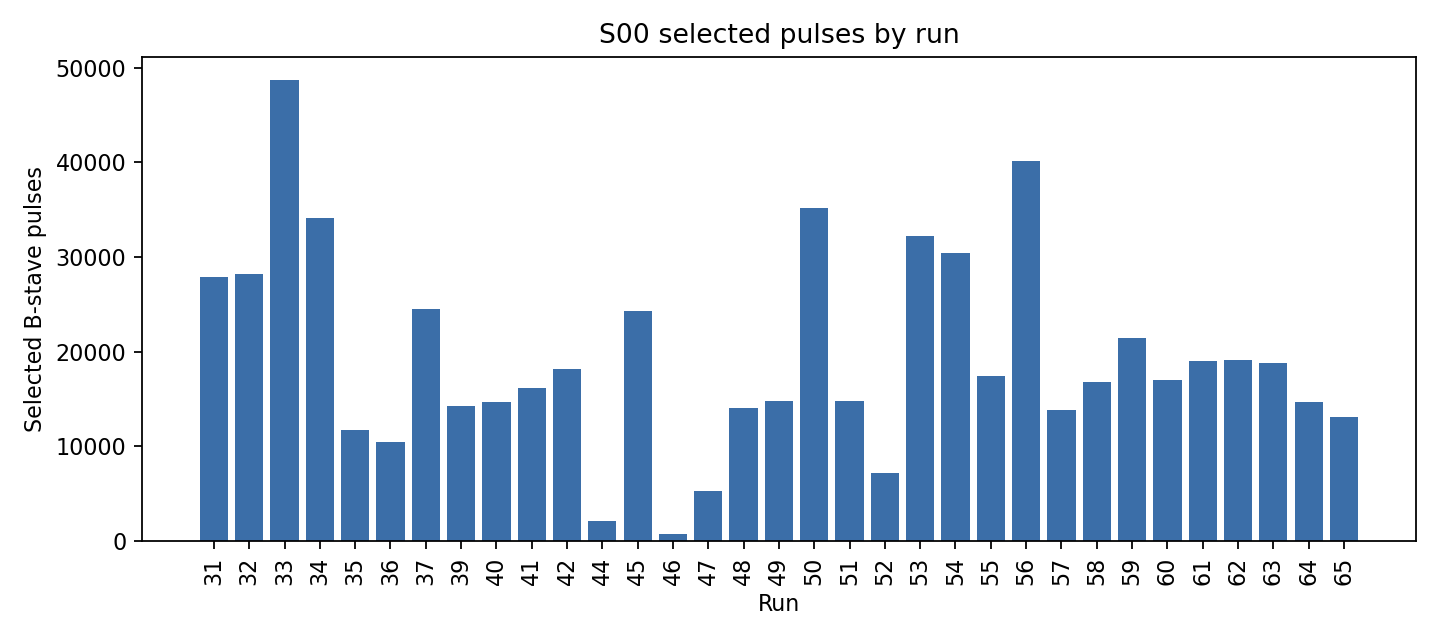
\includegraphics[width=0.48\textwidth]{../../reports/1780917628.449525.085b2dc0__s01b_s00_selected_table_manifest/fig_counts_by_run.png}
  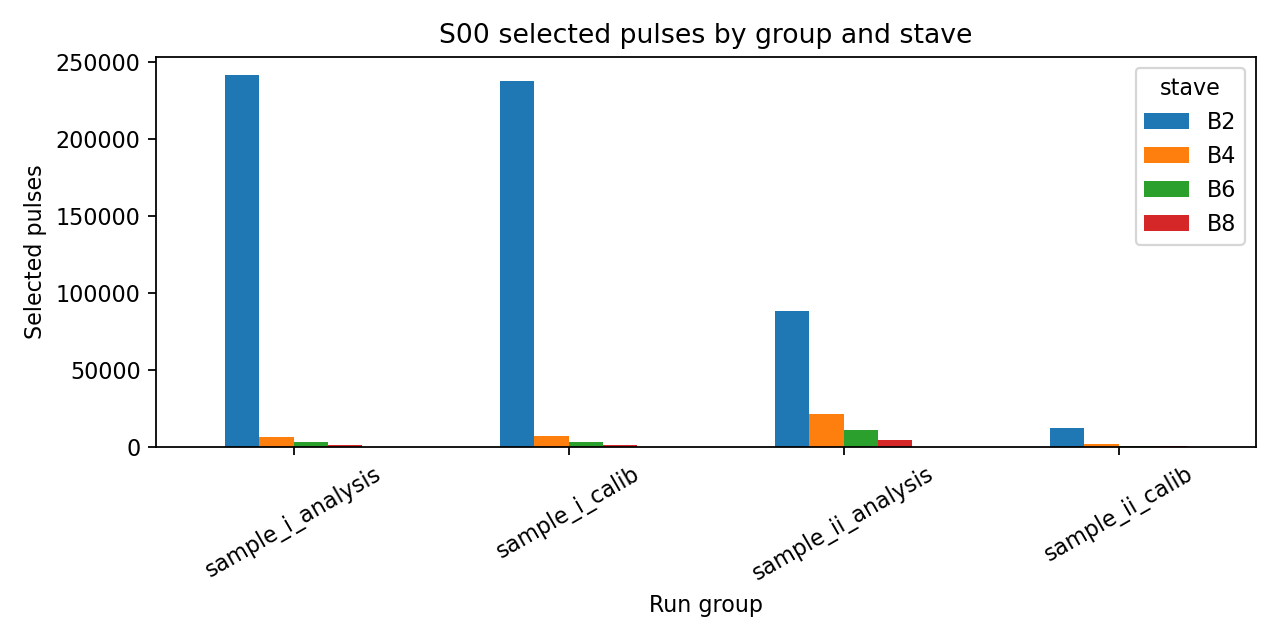
\includegraphics[width=0.48\textwidth]{../../reports/1780917628.449525.085b2dc0__s01b_s00_selected_table_manifest/fig_counts_by_group_stave.png}
  \caption{Selected-pulse count diagnostics from the S01b manifest.  Left:
  counts by run.  Right: group-by-stave composition after applying the physical
  even-channel convention.}
  \label{fig:s01b-counts}
\end{figure}

\section{Selection rule versus learned classifiers}
\label{sec:selection-ml}

The selection benchmark is intentionally asymmetric.  The traditional method is
the gate itself, Eq.~\ref{eq:s00-selection}; the machine-learning method is only
a sanity check that asks whether a classifier trained on summary features can
recover the same labels on held-out runs.  S00 and S01b used calibrated logistic
regression with amplitude, positive area, peak sample, and baseline features,
with runs 57 and 65 held out.  The model was well calibrated and nearly
perfect, but it was still inferior to the deterministic gate because the label
is the gate.

\begin{table}[H]
  \centering
  \small
  \caption{Run-held-out selection benchmark.  The deterministic threshold is
  the production method and wins.  The logistic model is retained only as a
  run-split sanity check.}
  \label{tab:selection-benchmark}
  \begin{tabular}{p{0.18\textwidth}p{0.28\textwidth}p{0.22\textwidth}p{0.22\textwidth}}
    \toprule
    Method family & Method & Metric & Value with 95\% CI \\
    \midrule
    Traditional & \(A>1000\) threshold & held-out accuracy & 1.000000 [1.000000, 1.000000] \\
    ML & calibrated logistic regression & held-out accuracy & 0.999796 [0.999491, 1.000000] \\
    \bottomrule
  \end{tabular}
\end{table}

The winner for selection is therefore the traditional deterministic threshold.
This conclusion is methodological as much as numerical: replacing an exact
definition by an approximate classifier would make the table less reproducible
without adding physics information.

\section{Amplitude-adaptive templates and \texorpdfstring{\(q_{\mathrm{template}}\)}{q-template}}
\label{sec:q-template}

After the selected table is fixed, S01 constructs an empirical pulse-shape
library.  Each selected waveform is baseline-subtracted, normalized by its peak
amplitude, and aligned on an 18-sample grid relative to the CFD20 crossing.
For stave \(s\) and amplitude bin \(k\), the traditional template is the
sample-wise median over calibration-run pulses,
\[
  T_{s,k,j} =
  \operatorname{median}_{e\in\mathcal{C}(s,k)} \tilde{y}_{e,j},
\]
where \(\tilde{y}\) denotes the aligned, amplitude-normalized waveform and
\(\mathcal{C}(s,k)\) contains calibration pulses in the stave and amplitude
bin.  Bins with fewer than 30 calibration pulses fall back to the stave-level
median.  The per-pulse template residual is
\[
  q_{\mathrm{template}}(e)
  =
  \left[
  \frac{1}{18}\sum_{j=0}^{17}
  \left(\tilde{y}_{e,j}-T_{s(e),k(e),j}\right)^2
  \right]^{1/2}.
  \label{eq:q-template}
\]
S01 writes \(q_{\mathrm{template}}\) for all \num{640737} selected pulses.
This scalar is not a truth label.  It is a compact residual describing how far
a pulse shape lies from its calibration-run stave/amplitude template.

\begin{figure}[H]
  \centering
  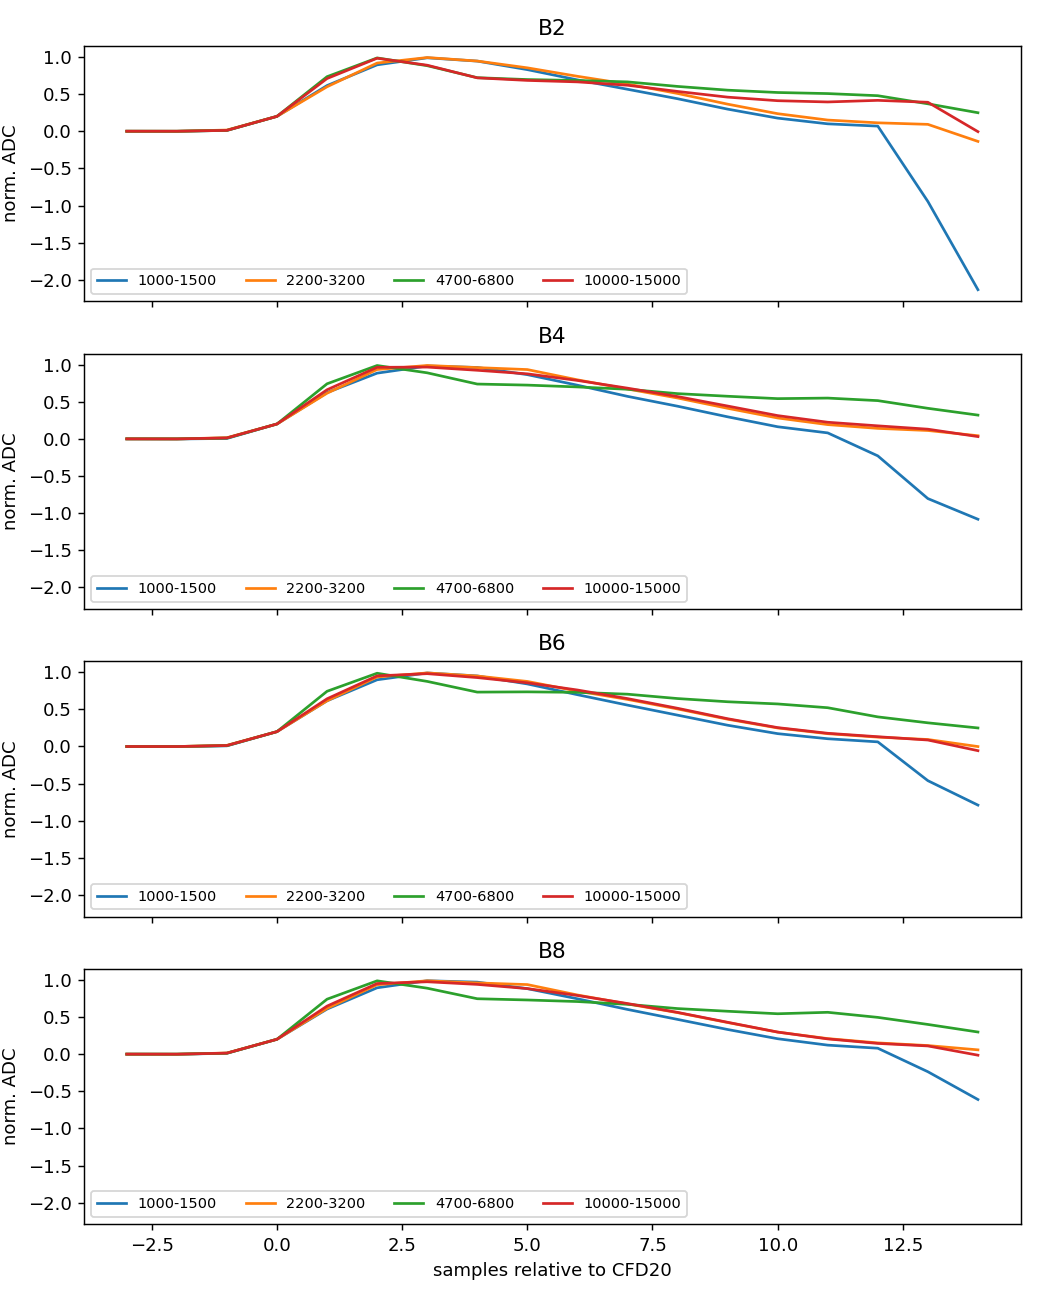
\includegraphics[width=0.48\textwidth]{../../reports/1780997954.15037.36463764__s01_full_dataset_templates/fig_template_library_examples.png}
  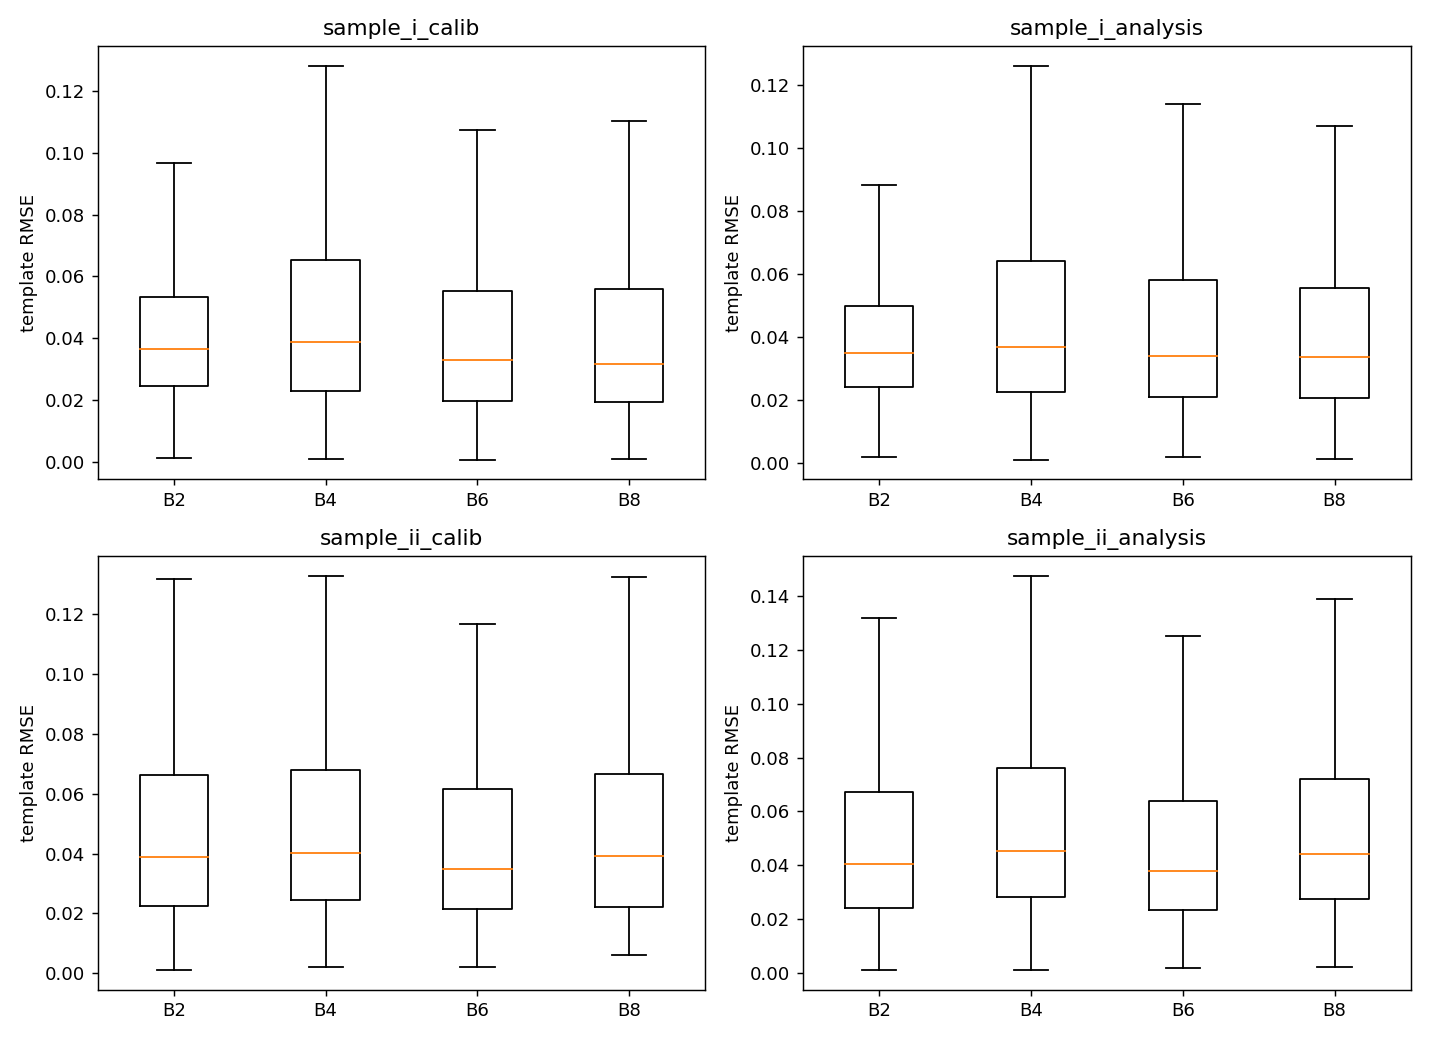
\includegraphics[width=0.48\textwidth]{../../reports/1780997954.15037.36463764__s01_full_dataset_templates/fig_q_template_by_group_stave.png}
  \caption{S01 amplitude-adaptive template outputs.  Left: examples from the
  empirical template library.  Right: \(q_{\mathrm{template}}\) distributions by
  group and stave for the full selected-pulse table.}
  \label{fig:s01-template-library}
\end{figure}

\section{Template benchmark: empirical median versus neural models}
\label{sec:template-benchmark}

S01 compared the empirical median template family with a fully connected
autoencoder trained only on calibration-run aligned waveforms.  Hyperparameters
were selected with grouped folds by run; the selected model used latent
dimension 8 and hidden dimension 32.  The benchmark metric was analysis-run
mean squared reconstruction residual on held-out analysis runs, with
run-bootstrap confidence intervals.  On this residual metric, the autoencoder
is the clear winner.

\begin{table}[H]
  \centering
  \small
  \caption{S01 held-out reconstruction benchmark for aligned, normalized pulse
  shapes.  Lower MSE is better.  Confidence intervals are 95\% run-bootstrap
  intervals over analysis runs.}
  \label{tab:s01-template-benchmark}
  \begin{tabular}{p{0.18\textwidth}p{0.32\textwidth}p{0.14\textwidth}p{0.26\textwidth}}
    \toprule
    Method family & Method & Metric & Value with 95\% CI \\
    \midrule
    Traditional & median stave/amplitude-bin template & MSE & 0.044414 [0.034249, 0.054782] \\
    NN & autoencoder, latent 8, hidden 32 & MSE & 0.002078 [0.001725, 0.002419] \\
    NN - traditional & difference & \(\Delta\)MSE & -0.042336 [-0.052421, -0.032381] \\
    \bottomrule
  \end{tabular}
\end{table}

The result is shown visually in Fig.~\ref{fig:s01-template-benchmark}.  The
neural model captures low-dimensional pulse-shape variation that is not
represented by fixed amplitude bins.  However, the S01 report correctly limits
the claim: the benchmark is reconstruction residual, not timing resolution,
particle identification, or absolute energy.  Downstream chapters evaluate
whether a lower waveform residual translates into a physics-facing observable.

\begin{figure}[H]
  \centering
  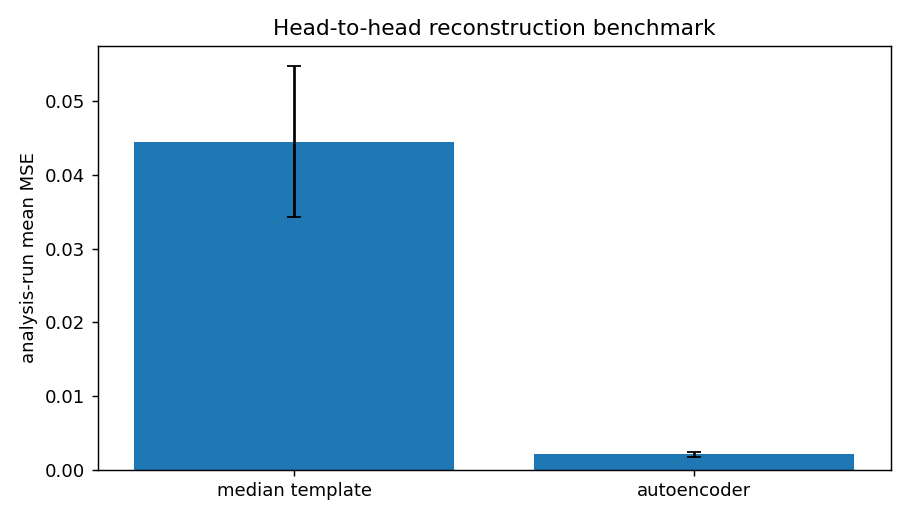
\includegraphics[width=0.72\textwidth]{../../reports/1780997954.15037.36463764__s01_full_dataset_templates/fig_template_vs_autoencoder_benchmark.png}
  \caption{S01 head-to-head reconstruction benchmark.  The autoencoder beats
  the empirical median template on held-out analysis-run MSE, but the result is
  interpreted as a shape-compression result rather than a physics calibration.}
  \label{fig:s01-template-benchmark}
\end{figure}

P10a tests a different neural architecture: a conditional MLP that maps stave
identity and log amplitude to an aligned normalized waveform template.  This
model improves a downstream phase-template timing metric but loses on the
primary \(q_{\mathrm{template}}\) MSE, and its shuffled-target control is a
warning that stave and amplitude alone do not define a stable held-out shape
generator.  For the reconstruction chapter, the empirical S01 template remains
the production definition of \(q_{\mathrm{template}}\).

\begin{table}[H]
  \centering
  \small
  \caption{P10a conditional-template stress test.  Lower is better for both
  metrics.  The primary \(q_{\mathrm{template}}\) metric favors the empirical
  amplitude-bin template; timing favors the conditional MLP but is treated as a
  downstream observation rather than a replacement for S01.}
  \label{tab:p10a-template-benchmark}
  \begin{tabular}{p{0.16\textwidth}p{0.27\textwidth}p{0.20\textwidth}p{0.27\textwidth}}
    \toprule
    Method family & Method & Metric & Value with 95\% CI \\
    \midrule
    Traditional & empirical amplitude-bin template & \(q\) MSE & 0.044414 [0.034222, 0.055344] \\
    NN & conditional MLP template & \(q\) MSE & 0.078062 [0.066158, 0.090569] \\
    NN - traditional & difference & \(\Delta q\) MSE & 0.033648 [0.027697, 0.041113] \\
    Traditional & empirical phase template & pairwise \(\sigma_{68}\) & 3.8306 ns [3.7325, 3.9344] \\
    NN & conditional MLP phase template & pairwise \(\sigma_{68}\) & 3.5789 ns [3.4857, 3.6801] \\
    NN - traditional & difference & \(\Delta\sigma_{68}\) & -0.2518 ns [-0.3781, -0.1331] \\
    \bottomrule
  \end{tabular}
\end{table}

\section{Amplitude-adaptive diagnostics in duplicate-readout closure}
\label{sec:p04c-closure}

The amplitude-adaptive template variables also appear in P04c, where the target
is the independent odd readout-side channel.  This is not an absolute energy
truth label, but it is a useful leakage-safe closure because the model inputs
use only the even physical-stave waveform and derived even-channel summaries;
run number, event number, and odd-channel samples are excluded.

P04c compares peak/integral baselines, fixed-bin template calibration,
adaptive-template scale, a stronger adaptive-template ridge, and a
histogram-gradient-boosted-tree regressor.  The strong traditional method is
the adaptive-template ridge, not the direct template scale.  Even so, the
gradient-boosted tree wins decisively on duplicate-readout closure.

\begin{table}[H]
  \centering
  \small
  \caption{P04c held-out duplicate-readout closure for runs 57 and 65.  Lower
  68th percentile absolute fractional error is better.  The winner is the
  gradient-boosted tree, but the interpretation is duplicate-readout closure,
  not absolute energy calibration.}
  \label{tab:p04c-closure}
  \begin{tabular}{p{0.14\textwidth}p{0.18\textwidth}p{0.34\textwidth}p{0.24\textwidth}}
    \toprule
    Target & Method family & Method & res68 with 95\% CI \\
    \midrule
    amplitude & Traditional & peak calibration & 0.1238 [0.1221, 0.1251] \\
    amplitude & Traditional & adaptive-template ridge & 0.0858 [0.0844, 0.0871] \\
    amplitude & ML & histogram-gradient-boosted trees & 0.00912 [0.00891, 0.00927] \\
    charge & Traditional & integral calibration & 0.1954 [0.1936, 0.1975] \\
    charge & Traditional & adaptive-template ridge & 0.1554 [0.1530, 0.1573] \\
    charge & ML & histogram-gradient-boosted trees & 0.0151 [0.0148, 0.0153] \\
    \bottomrule
  \end{tabular}
\end{table}

This closure result supports a broader pattern in the project.  Flexible ML
methods help when the task is a waveform-shape mapping to an independent
readout.  They should not be mistaken for detector truth when the target is
constructed from the same waveform or when no external energy/PID label exists.

\section{Systematic uncertainties and caveats}
\label{sec:data-systematics}

The dominant systematic risks in this chapter are not statistical fluctuations
of the selected count.  They are analysis-definition risks.

\begin{itemize}
  \item \textbf{Channel mapping.}  The selected table uses even raw channel
  blocks only.  Odd blocks are duplicate readout-side channels and belong in
  closure studies, not the production B-stave count.

  \item \textbf{Raw versus derived branches.}  The raw \texttt{HRDv} waveform
  rule is the selection authority.  Derived sorted \texttt{hrdMax} semantics do
  not reproduce the same gate and must not be used as a proxy for S00.

  \item \textbf{Processed-data availability.}  S01b found that the expected
  processed table was absent from the read-only data mirror in the sandbox.
  This is an infrastructure issue, not a physics discrepancy; the table is
  regenerated from raw ROOT and pinned by row count and checksum.

  \item \textbf{Template target semantics.}  \(q_{\mathrm{template}}\) is a
  reconstruction residual against a calibration-run empirical template.  It is
  not a truth label and not automatically a timing-quality, pile-up, or PID
  observable.

  \item \textbf{Run leakage.}  The quoted ML/NN comparisons use run-held-out or
  grouped-by-run validation.  This is essential because pulse shape, rate, and
  topology all vary by run and sample period.

  \item \textbf{Metric hierarchy.}  The autoencoder wins S01 reconstruction
  MSE, while the conditional MLP loses the primary P10a \(q\)-MSE but improves a
  timing metric.  The production choice therefore depends on the observable:
  empirical \(q_{\mathrm{template}}\) remains the transparent reconstruction
  variable; neural residuals are downstream candidates, not replacements for
  the selected-table definition.
\end{itemize}

\section{Chapter verdict}
\label{sec:data-verdict}

The selected data set is reproducible from raw ROOT: \num{640737} B-stave
pulses are recovered with zero count delta using the even-channel,
median-pedestal, \(A>1000\) ADC rule.  For selection, the traditional
deterministic threshold wins over calibrated logistic regression because it is
the exact definition and has held-out accuracy 1.000000.  For pulse-shape
reconstruction, the S01 autoencoder wins the held-out MSE benchmark over the
empirical amplitude-bin median template, with \(\Delta\mathrm{MSE}=-0.042336\)
and a 95\% CI entirely below zero.  For the production reconstruction record,
however, the empirical \(q_{\mathrm{template}}\) table remains the conservative
and interpretable artifact: it is tied to the exact S00 selected table, trained
only on calibration runs, and stress-tested against conditional neural
templates and duplicate-readout closure studies.

\chapter{Timing}
\emph{(chapter pending --- to be written by the fleet.)}

\chapter{Pile-up}
\label{chap:pileup}

\section{Scope and principal conclusion}
\label{sec:pileup_scope}

The pile-up studies ask a narrower question than a generic waveform-classifier
benchmark: how much of the high-current pulse population is consistent with
overlapping beam particles, what effective live-time should enter the rate
model, and whether learned waveform methods should replace the transparent
topology and template analyses.  The data contain no direct truth label for a
real pile-up pulse.  The analysis therefore separates three evidential layers:
first, current-dependent topology rates measured directly in the beam data;
second, raw-waveform live-time measurements that revise the effective time
window used in the Poisson occupancy calculation; and third, injected
two-pulse closure tests that rank reconstruction algorithms under a controlled
but synthetic truth definition.

The main physics conclusion is that the originally quoted maximum rate is
reproducible only as an assumption.  The S10 reproduction gives
$R_{\max}=4.222$ MHz when $\tau_{\mathrm{eff}}=90$ ns is inserted by hand.
However, the directly measured waveform live-time is materially longer:
the run-held-out template measurement gives a 10\% live-time of
$124.79$ ns with a 95\% bootstrap confidence interval
$[123.32,126.33]$ ns.  Rescaling the same occupancy limit with this
measured window gives
\begin{equation}
  R_{\max}^{\mathrm{meas}}
  =
  \frac{\mu_{\max}}{\tau_{\mathrm{live}}}
  =
  \frac{0.380}{124.79\ \mathrm{ns}}
  =
  3.05\ \mathrm{MHz},
  \label{eq:pileup_rmax_revision}
\end{equation}
not 4.22 MHz.  This is the central pile-up revision.

The method winner depends on the estimand.  For the beam-rate claim, the
winner is the traditional topology plus Poisson/live-time analysis: it is
transparent, directly tied to current and topology, and does not require a
synthetic label.  For template-like injected two-pulse decomposition, compact
neural methods, especially the MLP and the 18-sample one-dimensional CNN,
achieve lower timing RMS than the bounded two-pulse template fit.  That neural
advantage is not adopted as the beam-rate estimator because it comes with a
higher failure rate and because injected overlap truth is not real
high-current truth.

\section{Rate model and live-time definition}
\label{sec:pileup_rate_model}

The conventional occupancy calculation models the number of unresolved
particles in an effective live-time window as Poisson distributed.  If
$\mu=R\tau_{\mathrm{eff}}$ is the expected number of particles in the window,
then the no-more-than-one-particle probability is
\begin{equation}
  P(N \leq 1) = e^{-\mu}(1+\mu),
  \label{eq:pileup_poisson}
\end{equation}
and an allowed occupancy $\mu_{\max}$ maps to a maximum rate
\begin{equation}
  R_{\max} = \frac{\mu_{\max}}{\tau_{\mathrm{eff}}}.
  \label{eq:pileup_rmax}
\end{equation}
S10 reproduced the documented combined requirement $|dt|<1$ ns and
area $<20\%$ with $\mu_{\max}=0.380$.  With the historical
$\tau_{\mathrm{eff}}=90$ ns, this gives
$R_{\max}=4.222$ MHz.  The reproduction gate also recovered all six
low-current and high-current topology fractions within the predeclared
tolerance, so the discrepancy is not in event counting; it is in the
interpretation of the time window.

The S10b and S10c studies estimated the live-time directly from raw B-stack
waveforms.  For each held-out run, selected pulses were pedestal subtracted,
timed with CFD20, aligned by stave, and median combined.  The post-peak tail
was fit with
\begin{equation}
  y(t) = c + a \exp(-t/\tau),
  \label{eq:pileup_tail_fit}
\end{equation}
and the live-time was defined as the crossing below a chosen fraction of the
pulse amplitude.  A run-held-out ridge regressor from pulse-shape summaries to
the same live-time target was used as the ML comparison.  It excluded run,
event number, current labels, and direct last-above-threshold width features.

\begin{table}[H]
\centering
\caption{Measured waveform live-time and the implied rate revision.  Intervals
are 95\% bootstrap confidence intervals over held-out runs.  The traditional
method is the median-template exponential crossing; the ML method is the
run-held-out ridge live-time predictor.}
\label{tab:pileup_livetime}
\resizebox{\textwidth}{!}{%
\begin{tabular}{lrrrr}
\toprule
Threshold & Template live-time (ns) & Ridge live-time (ns) & $R_{\max}$ (MHz) & Above 90 ns? \\
\midrule
5\% & 141.06 [139.29, 143.01] & 124.75 [122.59, 126.69] & 2.69 & yes \\
10\% & 124.79 [123.32, 126.33] & 123.22 [120.71, 125.61] & 3.05 & yes \\
20\% & 101.87 [100.90, 102.83] & 119.18 [115.60, 122.48] & 3.73 & yes \\
Noise floor & 161.18 [158.76, 163.61] & 120.30 [117.03, 123.22] & 2.36 & yes \\
\bottomrule
\end{tabular}
}
\end{table}

The threshold scan is important because it tests whether the 90 ns value could
be recovered by a reasonable alternative crossing definition.  It could not:
even the shortest traditional crossing, the 20\% threshold, has its lower
bootstrap bound above 100 ns.  The ridge predictor broadly agrees with the
10\% result but is not the primary rate estimator, since the template crossing
is simpler and closer to the physical definition of an unresolved pulse tail.

\begin{figure}[H]
\centering
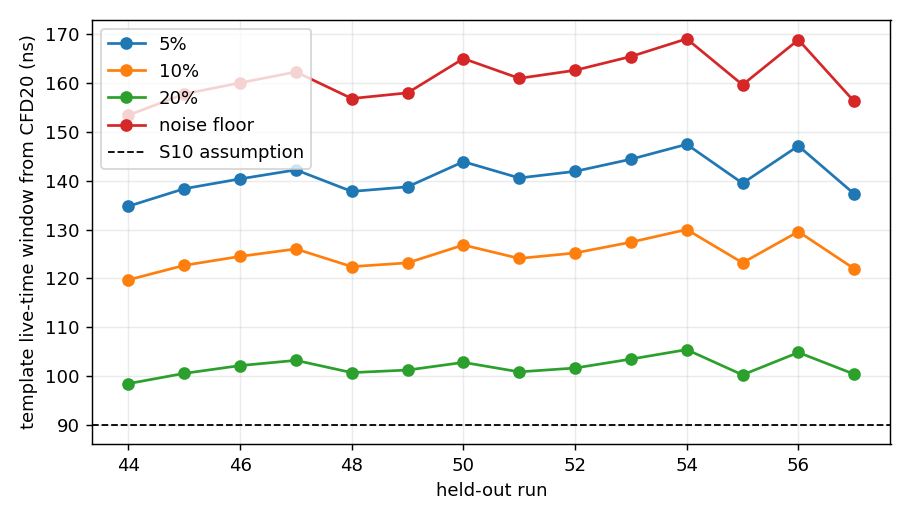
\includegraphics[width=0.92\textwidth]{../figures/reports/1781007337.1308.7dc86005/fig_threshold_scan_by_run.png}
\caption{Run-held-out live-time threshold scan from S10c.  All scanned
template definitions remain above the historical 90 ns assumption.}
\label{fig:pileup_threshold_scan}
\end{figure}

\section{Current-dependent topology excess}
\label{sec:pileup_current_topology}

The beam-current comparison uses selected B-stave events as the denominator.
Runs 46 and 47 form the 2 nA reference, while runs 44, 45, and 48--57 form the
20 nA sample.  The most interpretable traditional observable is the downstream
topology fraction per selected event.  S10 measured a rise from 2.312\% at
2 nA to 3.341\% at 20 nA, a high-minus-low excess of 1.029 percentage points
with a 95\% binomial confidence interval of [0.637, 1.421] percentage points.
Equivalently, about 30.8\% of the high-current downstream rate is attributable
to the current-dependent excess under this topology definition.

\begin{table}[H]
\centering
\caption{S10 current-topology reproduction.  Fractions are per selected event
and reproduce the documented values within the predeclared 0.0015 tolerance.}
\label{tab:pileup_topology}
\begin{tabular}{lrrr}
\toprule
Observable & 2 nA & 20 nA & High/low ratio \\
\midrule
Multi-stave fraction & 0.015588 & 0.026806 & 1.720 \\
$\geq 3$-stave fraction & 0.004111 & 0.008538 & 2.077 \\
Downstream fraction & 0.023124 & 0.033414 & 1.445 \\
\bottomrule
\end{tabular}
\end{table}

The corresponding ML diagnostic in S10 was an injection-trained logistic
pile-up score using waveform-shape features such as area-to-peak ratio, tail
fractions, late fractions, early fractions, width handles, and post-peak
structure.  It was trained on synthetic clean versus injected two-pulse
waveforms, not on real beam pile-up truth.  On real selected pulses the
low-current-trained score mean rose from 0.1213 to 0.1574, a high/low ratio of
1.297.  This confirms that waveform morphology changes with current, but the
ratio is much smaller than the beam-current ratio and remains a proxy rather
than a calibrated pile-up probability.

\begin{figure}[H]
\centering
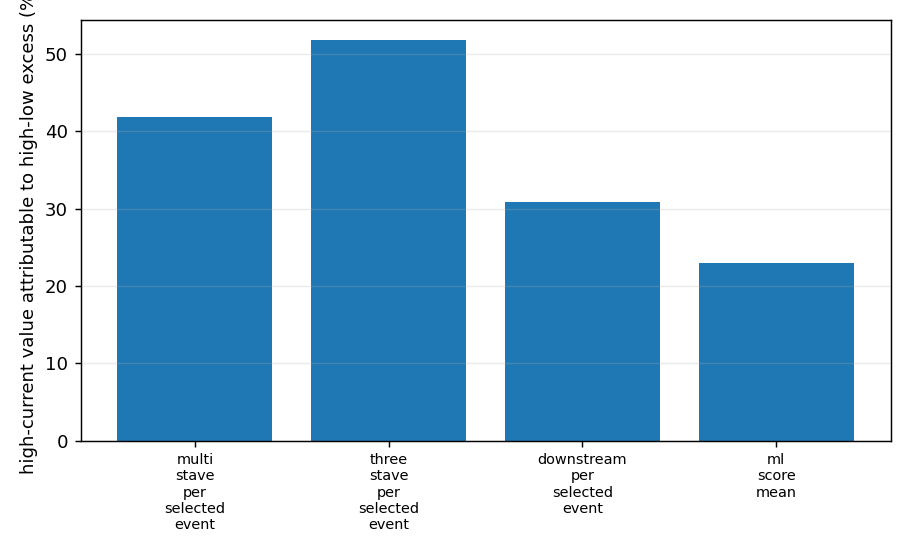
\includegraphics[width=0.86\textwidth]{../figures/reports/1780997954.15277.548b01a3__s10_pileup_rate_model/fig_current_excess.png}
\caption{S10 current-dependent excess.  The topology observable gives the
physics-facing current-rate handle; waveform ML scores are used as diagnostics
of morphology rather than direct rate estimators.}
\label{fig:pileup_current_excess}
\end{figure}

\section{Two-pulse reconstruction benchmark}
\label{sec:pileup_two_pulse}

The two-pulse studies provide controlled algorithm rankings under a synthetic
truth definition.  The construction uses S01-style empirical B-stack templates
and real single-pulse residuals from raw selected pulses.  Training uses runs
58--62 and evaluation holds out runs 63 and 65.  The traditional reconstruction
is a bounded two-pulse template fit: it initializes with CFD20, scans first
pulse timing offsets and fixed separation hypotheses, solves amplitudes and
baseline by least squares, and records constrained-fit failures.  The neural
comparators are compact waveform models trained on the same injected mixtures:
an MLP classifier/regressor for overlap probability, two times, and two
amplitudes, and a compact 18-sample one-dimensional CNN with convolutional
feature extraction and the same decomposition heads.

For a waveform $x(t)$, the traditional model is
\begin{equation}
  x(t) = b + A_1 T(t-t_1) + A_2 T(t-t_2) + \epsilon(t),
  \label{eq:pileup_two_pulse_template}
\end{equation}
with a template $T$ built only from training runs.  The fit minimizes the
sum of squared residuals over the scanned hypotheses.  The neural models
replace the explicit hypothesis scan with learned functions
$f_{\theta}(x)=(\hat p,\hat t_1,\hat t_2,\hat A_1,\hat A_2)$, optimized on
injected mixtures from the training runs.

\begin{table}[H]
\centering
\caption{Injected two-pulse reconstruction benchmark.  Intervals are 95\%
bootstrap intervals over held-out run blocks.  The neural methods win on time
RMS and AP, while the traditional fit wins on failure rate.}
\label{tab:pileup_two_pulse}
\resizebox{\textwidth}{!}{%
\begin{tabular}{lrrrr}
\toprule
Method & AP & Time RMS (ns) & Charge res68 & Failure rate \\
\midrule
Bounded two-pulse template fit & 0.767 [0.737, 0.796] & 13.30 [12.00, 14.56] & 0.098 [0.089, 0.109] & 0.168 [0.139, 0.200] \\
Compact MLP & 0.851 [0.820, 0.879] & 10.67 [9.62, 11.84] & 0.078 [0.068, 0.084] & 0.295 [0.261, 0.331] \\
Compact 18-sample CNN & 0.868 [0.864, 0.874] & 10.01 [9.88, 10.14] & 0.080 [0.075, 0.085] & 0.228 [0.220, 0.237] \\
\bottomrule
\end{tabular}
}
\end{table}

S10d also translated the recovery benchmark into a resolvability live-time:
the first tested separation after which all larger separations satisfy
\begin{equation}
  |\mathrm{median\ timing\ bias}| < 1\ \mathrm{ns},
  \qquad
  |\mathrm{median\ total\ area\ bias}| < 0.20 .
  \label{eq:pileup_resolvability_criteria}
\end{equation}
Under this definition, the
bounded template fit becomes resolvable at 60 ns with bootstrap interval
[40, 60] ns, while the compact MLP reaches 20 ns with interval [15, 60] ns.
The point estimate favors ML, but the upper confidence limit overlaps the
template fit and the MLP failure rate is almost twice as large.

\begin{figure}[H]
\centering
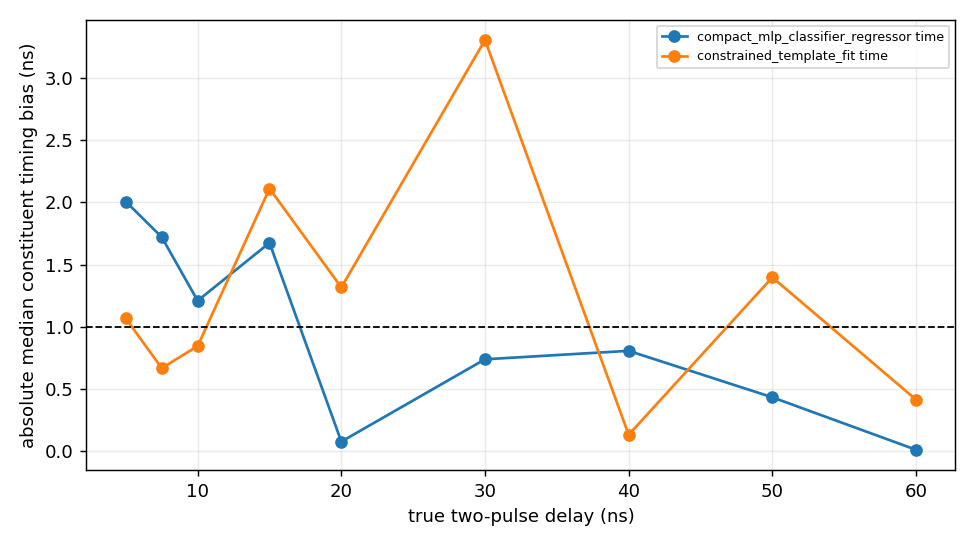
\includegraphics[width=0.88\textwidth]{../figures/reports/1781007337.1325.2241031c/fig_resolvability_delay_bias.png}
\caption{S10d resolvability-delay bias curves for the bounded template fit and
compact MLP.  Neural reconstruction reaches the bias criterion at a shorter
point estimate, but the operational interpretation is limited by failure rate
and synthetic injection truth.}
\label{fig:pileup_resolvability}
\end{figure}

\section{Failure-aware abstention}
\label{sec:pileup_abstention}

Average timing RMS is not sufficient for a production pile-up correction.  A
method that gives excellent estimates for many events but silently fails on a
large tail can bias downstream timing or charge analyses.  P05b therefore
calibrated abstention gates on the S11a injected benchmark.  Bad recovery was
defined as a base-method failure, constituent-time RMS above 12 ns, or absolute
charge bias above 0.20.  The traditional gate used train-run-only cuts on fit
failure, fractional SSE improvement, a $\chi^2/\mathrm{ndf}$ proxy, fitted
separation, and amplitude ratio.  The ML gate used an isotonic-calibrated
logistic risk model over normalized waveform features and fit diagnostics.

\begin{table}[H]
\centering
\caption{P05b failure-aware operating points.  The traditional gate is more
selective and safer among accepted events; the ML gate keeps more coverage but
accepts a higher bad-recovery rate.}
\label{tab:pileup_abstention}
\resizebox{\textwidth}{!}{%
\begin{tabular}{lrrrr}
\toprule
Gate & Coverage & Accepted RMS (ns) & Charge res68 & Bad recovery \\
\midrule
Traditional quality cuts & 0.343 & 7.42 [6.61, 8.26] & 0.070 [0.067, 0.075] & 0.092 [0.082, 0.104] \\
ML isotonic failure gate & 0.728 & 8.44 [8.28, 8.59] & 0.064 [0.064, 0.069] & 0.144 [0.131, 0.157] \\
\bottomrule
\end{tabular}
}
\end{table}

This result explains why the chapter does not promote the neural decomposers
as the pile-up correction by default.  The CNN and MLP are the timing-RMS
winners on injected overlaps, but the traditional quality gate provides a
lower-risk accepted sample.  The practical conclusion is an operating-point
trade-off: neural recovery is useful for diagnostic studies and perhaps for
high-coverage correction studies, while conservative template-quality cuts are
safer when a low bad-recovery rate is the controlling requirement.

\begin{figure}[H]
\centering
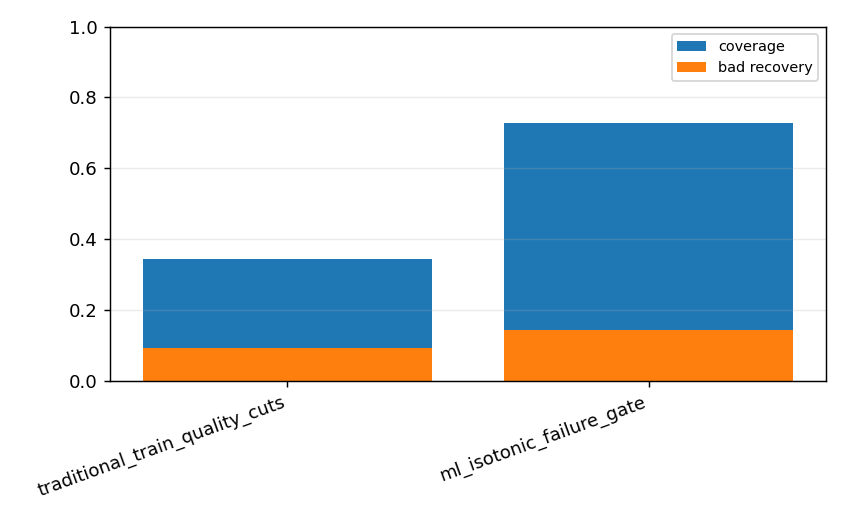
\includegraphics[width=0.82\textwidth]{../figures/reports/1781014241.437.0e0024cb/fig_gate_coverage_bad_rate.png}
\caption{P05b risk-coverage comparison for failure-aware two-pulse recovery.
The ML gate buys coverage; the traditional gate buys a cleaner accepted
sample.}
\label{fig:pileup_abstention}
\end{figure}

\section{CWoLa current-scaling diagnostic}
\label{sec:pileup_cwola}

S13b tested whether a weakly supervised current classifier could reproduce the
S10 waveform-score current scaling under independent run transfer.  The method
is Classification Without Labels: train a classifier to distinguish mixtures
of high-current and low-current selected pulses, then interpret the learned
score as a morphology-sensitive current discriminator rather than as a
per-pulse truth label.  The CWoLa model was a random forest trained on
normalized waveform samples plus pulse-shape summaries.  It excluded run,
event number, current labels as features, and downstream/topology labels.

The split was by run block.  The A-to-B fold trained on low run 46 plus high
runs 44, 45, and 48--51, then tested on low run 47 plus high runs 52--57.  The
B-to-A fold reversed the partition.  Bootstrap intervals resampled held-out
runs within current group; with only two low-current runs, the low-current
component is necessarily a limited systematic.

\begin{table}[H]
\centering
\caption{S13b current-scaling comparison.  CWoLa transfers as a modest
waveform-shape current discriminator, but the topology ratio remains the
stronger physics-facing rate handle.}
\label{tab:pileup_cwola}
\begin{tabular}{lrr}
\toprule
Method & High/low score or rate ratio & Held-out current AUC \\
\midrule
Single traditional shape feature & 1.064 [0.982, 1.095] & 0.633 [0.346, 0.748] \\
CWoLa random forest shape score & 1.220 [1.193, 1.257] & 0.668 [0.656, 0.682] \\
Shuffled-label random forest & 1.020 [1.012, 1.032] & 0.559 [0.538, 0.590] \\
Traditional downstream topology & 1.445 [1.220, 2.542] & -- \\
\bottomrule
\end{tabular}
\end{table}

\begin{figure}[H]
\centering
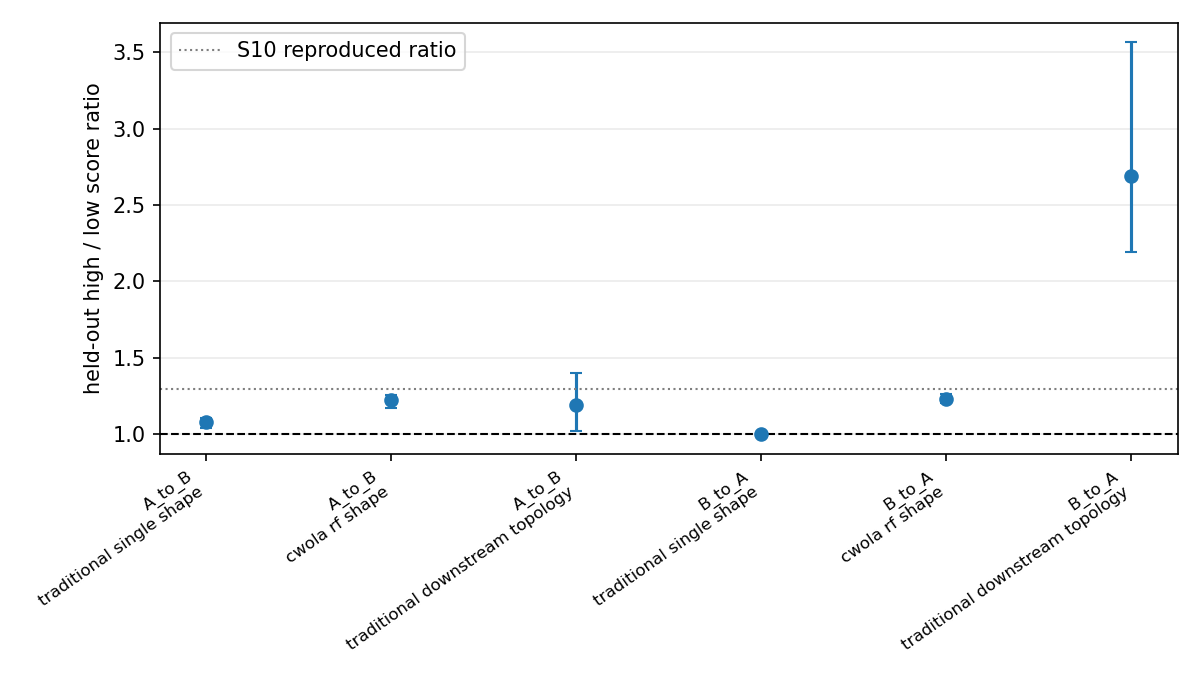
\includegraphics[width=0.86\textwidth]{../figures/reports/1781000867.546938.20f0173c/fig_run_block_score_ratios.png}
\caption{S13b run-block score ratios.  The CWoLa score transfers beyond the
S10 two-low-run reference, but its magnitude is smaller than the topology
ratio and should be interpreted diagnostically.}
\label{fig:pileup_cwola}
\end{figure}

\section{Systematics and caveats}
\label{sec:pileup_systematics}

The dominant systematic is the absence of real pile-up truth.  Current
dependence is directly measured, but individual pulses are not labeled as
single-particle or multi-particle beam events.  Therefore the topology excess
and Poisson/live-time calculation support a rate revision, whereas the MLP,
CNN, ridge, and CWoLa models support algorithmic or diagnostic statements.

The live-time systematic is definitional.  A 10\% threshold gives the
headline 3.05 MHz revision, but a 20\% threshold gives 3.73 MHz and a
noise-floor threshold gives 2.36 MHz.  All reasonable scanned definitions are
longer than 90 ns, so the qualitative revision is stable even though the exact
rate depends on the chosen crossing.  This uncertainty should be propagated as
a live-time-definition envelope rather than hidden inside a single nominal
number.

The injection systematic affects the two-pulse reconstruction winner.  The
injected mixtures use empirical templates and real residuals, but they are
still generated from the same template family used by the reconstruction
benchmark.  Real high-current pile-up can include saturation, baseline
excursions, broad-late pulse shapes, and topology effects that are not fully
represented.  Strict run splits, event-overlap checks, and shuffled-label
sentinels reduce leakage risk, but they cannot convert injected truth into
measured beam truth.

Finally, the high-current excess is heterogeneous.  Follow-up studies find
that after matching on amplitude, baseline, and topology the excess
concentrates in high-amplitude, large-baseline-lowering, broad-late pulses.
This heterogeneity is precisely why topology remains the rate handle and ML
scores remain monitors: a scalar waveform score can detect current-sensitive
morphology, but it does not by itself identify a clean Poisson pile-up
component.

\section{Chapter verdict}
\label{sec:pileup_verdict}

For the pile-up rate model, the traditional analysis wins.  The reproducible
occupancy equation gives 4.222 MHz only under the historical 90 ns assumption;
the measured waveform live-time revises the preferred 10\% estimate to
3.05 MHz, with a threshold-definition envelope spanning roughly
2.36--3.73 MHz in the S10c scan.  For injected two-pulse recovery, neural
methods win the timing-RMS benchmark: the compact MLP reaches 10.67 ns and the
18-sample CNN reaches 10.01 ns, compared with 13.30--13.90 ns for the bounded
template fit.  But the bounded fit and its train-derived quality cuts remain
the safer operational choice when bad-recovery rate is the controlling
criterion.  CWoLa random forests provide a useful current-scaling diagnostic
with a high/low ratio of 1.220 and held-out AUC of 0.668, but they do not
replace the downstream topology ratio of 1.445 as the physics-facing evidence.

\chapter{Pulse Shape and Learned Representations}

\section{Physics question and data scope}

The B-stack waveform has only 18 samples per readout channel, but those samples encode several
distinct effects: the prompt scintillation pulse, electronics shaping, baseline excursions,
late charge, saturation, and occasional malformed or overlapping pulses.  This chapter
summarises the studies that asked whether learned waveform representations expose useful
structure beyond transparent shape variables.  The emphasis is deliberately conservative:
learned embeddings are useful only if they survive the same run-held-out and leakage-sentinel
standards used elsewhere in the analysis.

The recurring raw-data gate is the S00 B-stave selection.  For a waveform $x_{e,c,s}$ from event
$e$, channel $c$, and sample $s$, the pedestal-subtracted pulse is
\begin{equation}
  y_{e,c,s} = x_{e,c,s} - {\rm median}\{x_{e,c,0},x_{e,c,1},x_{e,c,2},x_{e,c,3}\},
  \qquad A_{e,c} = \max_s y_{e,c,s}.
\end{equation}
The selected B-stack pulse table keeps the even B-stave channels B2, B4, B6, and B8 when
$A_{e,c}>1000$ ADC.  The full gate reproduces 640737 selected pulse records from raw ROOT in
the P01 and P09 studies before fitting any representation or anomaly model.  The P02 discovery
study reused the same gate on a 60000-pulse subset of runs 50 and 58--65.

\section{Traditional and learned representations}

The traditional representation is principal component analysis (PCA) of amplitude-normalised
waveforms, optionally augmented by hand-engineered shape summaries such as peak sample, area,
late fraction, width, plateau, asymmetry, and template residuals.  PCA provides the linear
rank-$k$ approximation
\begin{equation}
  \hat{z}_i^{\rm PCA}(k) = \bar{z} + U_k U_k^{T}(z_i-\bar{z}),
  \qquad
  {\cal L}_{\rm rec} = \frac{1}{18N}\sum_i \lVert z_i-\hat{z}_i\rVert_2^2 ,
\end{equation}
where $z_i$ is the normalised 18-sample pulse.  The learned comparator is a compact autoencoder,
either a plain fully connected autoencoder in the P02 discovery study or a masked-denoising
autoencoder in P01.  In the latter case, random samples are masked during training and the network
minimises the same reconstruction loss while learning a bottleneck representation
\begin{equation}
  h_i=f_\theta(z_i), \qquad \hat{z}_i=g_\phi(h_i), \qquad
  \min_{\theta,\phi} \sum_i \lVert z_i-g_\phi(f_\theta(\tilde{z}_i))\rVert_2^2 .
\end{equation}

\begin{table}[H]
\centering
\caption{Representation benchmarks on held-out or discovery samples.  P01 intervals are
95\% run-block bootstrap CIs on held-out runs 42, 57, 64, and 65.  P02 is an unsupervised
60000-pulse discovery benchmark without a predictive run split; it is therefore used as
representation evidence, not as a downstream physics claim.}
\begin{tabular}{llrrrr}
\toprule
Study & Method & Latent dim. & Metric & Value & 95\% CI \\
\midrule
P01 & PCA & 4 & recon. MSE & 0.01337 & [0.00922, 0.01696] \\
P01 & masked AE & 4 & recon. MSE & 0.01428 & [0.01030, 0.01772] \\
P01 & hand-shape probe & -- & balanced acc. & 0.3527 & [0.3227, 0.3650] \\
P01 & AE-4 probe & 4 & balanced acc. & 0.3638 & [0.3446, 0.3707] \\
P02 & PCA & 2 & recon. MSE & 0.02622 & -- \\
P02 & AE & 2 & recon. MSE & 0.01294 & -- \\
P02 & PCA & 4 & recon. MSE & 0.00880 & -- \\
P02 & AE & 4 & recon. MSE & 0.00527 & -- \\
P02 & PCA & 8 & recon. MSE & 0.00166 & -- \\
P02 & AE & 8 & recon. MSE & 0.00292 & -- \\
\bottomrule
\end{tabular}
\end{table}

The resulting picture is not a simple ``ML wins'' statement.  At very low dimension the
nonlinear AE is clearly more compact in P02, improving reconstruction MSE by 50.6\% at
dimension 2, 40.6\% at dimension 3, and 40.1\% at dimension 4.  At dimension 8, however, linear
PCA is already close to lossless for this detector waveform and beats the small AE.  P01's
strict run-held-out benchmark reaches the same qualitative conclusion from the opposite
direction: the masked AE is a useful compact nonlinear embedding, but PCA and hand-shaped
features remain strong baselines.  The downstream stave probe improves only from 0.3527 to
0.3638 balanced accuracy, and the interval overlap means it should not be read as a robust
physics win.

\begin{figure}[H]
\centering
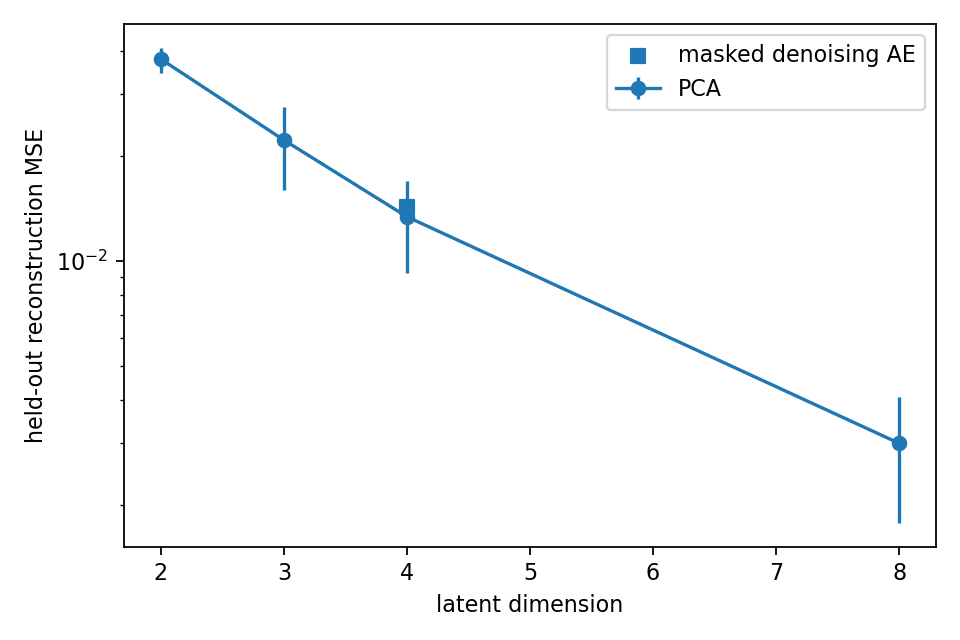
\includegraphics[width=0.92\textwidth]{../figures/reports/1780997954.15517.0cbc248c__p01_self_supervised_waveform_representation/fig_reconstruction_head_to_head.png}
\caption{P01 held-out reconstruction comparison between PCA and the masked-denoising
autoencoder.  The run-held-out split protects the reconstruction and probe summaries from
same-run leakage.}
\end{figure}

\begin{figure}[H]
\centering
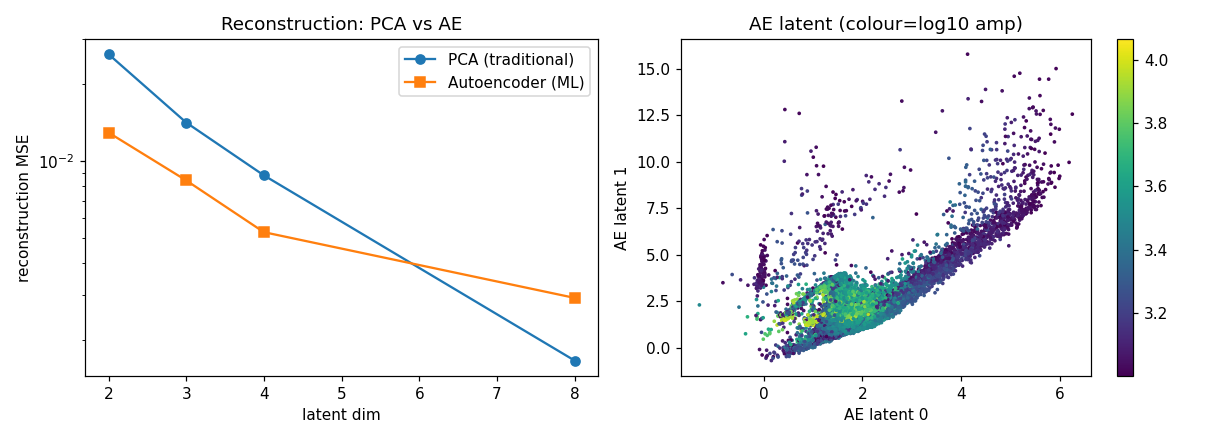
\includegraphics[width=0.92\textwidth]{../figures/reports/P02_pulse_representation_discovery/fig_pca_vs_ae_and_latent.png}
\caption{P02 compact-representation scan and latent map.  The AE is best at dimensions 2--4,
while PCA dominates once eight linear components are allowed.}
\end{figure}

\section{Unsupervised pulse types}

P02 used the AE latent space for label-free clustering.  The first eight PCA components already
explain 99.7\% of the waveform variance, but the low-dimensional AE map separates a small
morphology that is not obvious from amplitude alone.  K-means with five clusters on the AE-3
latent found two dominant normal pulse groups, peaking at samples 7--8, and an early-peak class
with peak sample near 3, low amplitude, and near-zero or pathological integrated area.  The
early-peak clusters account for about 2640 of 60000 pulses, or roughly 4.4\% of the discovery
sample.

\begin{table}[H]
\centering
\caption{P02 AE-cluster interpretation.  Counts are from the 60000-pulse discovery subset.}
\resizebox{\textwidth}{!}{%
\begin{tabular}{lrrrl}
\toprule
Cluster family & Clusters & Pulses & Median peak sample & Interpretation \\
\midrule
Normal, higher amplitude & 2 & 24201 & 7 & Ordinary late-positive pulse family \\
Normal, lower amplitude & 3 & 25137 & 8 & Ordinary lower-amplitude pulse family \\
Intermediate shape & 0 & 8025 & 5 & Mixed prompt/late morphology \\
Early-peak anomalous & 1, 4 & 2637 & 3 & Low-area early peak / pretrigger-like atom \\
\bottomrule
\end{tabular}
}
\end{table}

\begin{figure}[H]
\centering
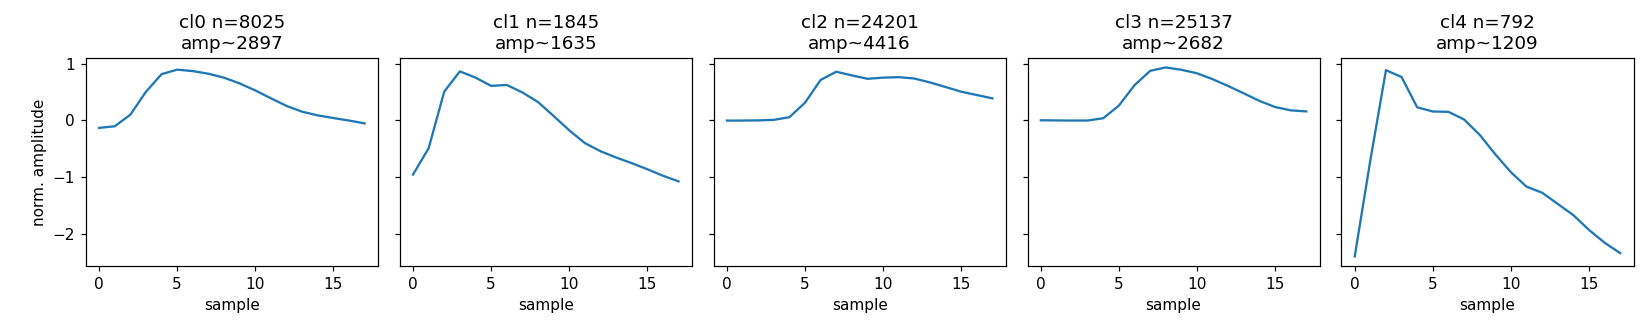
\includegraphics[width=0.92\textwidth]{../figures/reports/P02_pulse_representation_discovery/fig_cluster_mean_waveforms.png}
\caption{Mean waveforms for P02 latent clusters.  The early-peak family was found without
labels and motivated the later anomaly-taxonomy studies.}
\end{figure}

This is one of the strongest positive uses of representation learning in the pulse-shape
program: not a black-box classifier, but a hypothesis generator that exposes a coherent waveform
atom for later audits.  It also illustrates the limit of unsupervised evidence.  Cluster labels
are inferred from waveform morphology and cross-tabulations; they are not particle species,
pile-up truth, or timing truth.

\section{Rare waveform anomaly taxonomy}

P09 turned the P02 discovery into a held-out anomaly audit.  The traditional method ranked
pulses by robust train-run template residuals and transparent shape scores, including
\texttt{q\_template}, peak sample, late fraction, baseline residual, saturation count,
duplicate-channel timing span, secondary peak, and undershoot.  The learned method combined PCA
reconstruction error, AE reconstruction error, and an IsolationForest density score in PCA+AE
latent space.  The gallery was balanced by held-out run and stave, while identifiers were
excluded from scoring features.

\begin{table}[H]
\centering
\caption{P09a top-128 anomaly gallery audit on held-out runs.  Intervals are 95\% bootstrap CIs
over held-out runs.}
\begin{tabular}{lrrr}
\toprule
Method & Curated precision & Novel precision & Duplicate-event rate \\
\midrule
Robust template ranker & 0.898 [0.852, 0.945] & 0.555 [0.508, 0.625] & 0.0156 [0, 0.0469] \\
PCA+AE+IsolationForest & 0.883 [0.797, 0.969] & 0.766 [0.703, 0.828] & 0.0469 [0, 0.0938] \\
Balanced random & 0.180 [0.125, 0.242] & 0.164 [0.109, 0.227] & 0.0166 [0, 0.0473] \\
\bottomrule
\end{tabular}
\end{table}

The traditional ranker has the slightly higher curated precision, while the learned ranker is
substantially better for novel taxa.  This is a useful and interpretable division of labour:
robust template scores are good at recovering known curated failures, whereas the latent-density
score is better at surfacing morphology that was not already encoded by the hand score.  The
dominant held-out taxa were unassigned common pulses (91.5\%), novel early-pretrigger pulses
(4.02\%), novel delayed peaks (2.65\%), baseline excursions (1.23\%), and a much smaller
broad-template-mismatch class (0.272\%).

P09c then asked whether delayed-peak and broad-template-mismatch taxa propagate into timing,
charge, baseline, or pile-up sentinels.  For the delayed-peak target, the learned latent-isolation
score separated the target stratum much more effectively than the frozen robust-template score
(average precision 0.789 versus 0.433).  The same target had a large pile-up-score displacement
of 14.66 with CI [14.60, 14.70], a charge-bias delta of -4.82 with CI [-4.95, -4.65], and no
timing-tail or baseline-excursion enrichment under the frozen definitions.  The broad-template
class had only 162 held-out targets and one veto-like positive, so its perfect recover-veto AP in
one ML row is explicitly low-evidence and not a robust operational result.

\section{Downstream value and leakage sentinels}

The strongest caveat is that a good latent space is not automatically a good physics observable.
P01c and P01e repeatedly tested whether AE latents improve downstream waveform probes after
stricter controls.  In P01c, residual hand/PCA features reached balanced accuracy 0.331
[0.304, 0.349] on a leakage-sentinel task, while residual AE-4 reached only 0.235
[0.221, 0.246].  The amplitude/topology proxy and target-topology leakage sentinel were much
larger than either representation, showing how easily a representation claim can be dominated by
detector topology rather than pulse shape.  In P01e's strict timing audit, traditional hand-shape
ridge and AE-latent ridge were effectively tied: $\sigma_{68}=1.962$ ns [1.882, 2.064] for the
traditional model and $\sigma_{68}=1.965$ ns [1.885, 2.058] for the AE latent.

\begin{figure}[H]
\centering
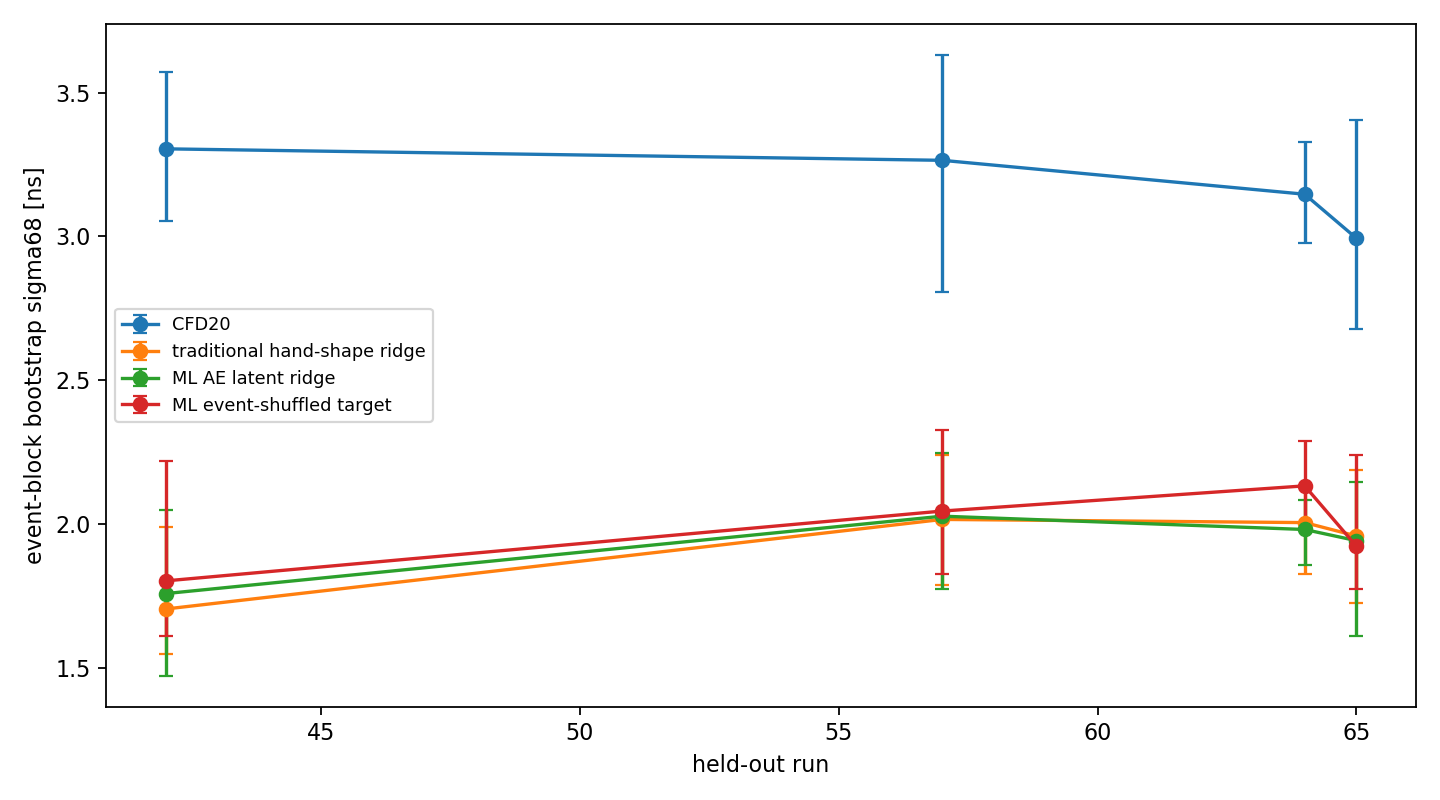
\includegraphics[width=0.86\textwidth]{../figures/reports/1781010798.1019.19c63d1a__p01e_strict_latent_timing_audit/fig_loro_sigma68.png}
\caption{P01e strict leave-one-run-out timing audit.  AE latents match but do not beat the
traditional hand-shape ridge once amplitude-bin shortcuts are removed.}
\end{figure}

The adopted rule is therefore asymmetric.  Latent representations are acceptable for discovery,
triage, and compact visualisation.  They are not accepted as independent physics improvements
unless the ML interval beats the traditional interval under run-held-out evaluation and remains
above repeated shuffled-label and run/topology sentinels.

\section{Systematics and caveats}

\begin{table}[H]
\centering
\caption{Main systematic controls for pulse-shape representation studies.}
\resizebox{\textwidth}{!}{%
\begin{tabular}{lll}
\toprule
Risk & Control & Residual caveat \\
\midrule
Same-run leakage & Held-out runs 42, 57, 64, 65 in P01/P09 & P02 discovery has no predictive split \\
Topology proxy & Amplitude-only and topology-mask sentinels & Stave labels are not particle truth \\
Overinterpreted clusters & Freeze taxa, then audit matched held-out rows & Cluster meaning remains morphological \\
Tiny anomaly support & Run-block bootstrap and positive-count audits & Broad-mismatch veto evidence is sparse \\
Black-box novelty & Compare to robust template ranker & ML novelty is triage, not final adjudication \\
\bottomrule
\end{tabular}
}
\end{table}

Several limitations follow directly from these controls.  First, the 18-sample pulse is
low-dimensional enough that a strong linear baseline is hard to beat when more than a few
components are allowed.  Second, some labels used for probes are detector or taxonomy labels, not
external truth labels.  Third, the most interesting anomaly taxa are rare, so their operational
impact must be propagated through timing, charge, and pile-up analyses rather than inferred from
gallery precision alone.  Finally, no representation result here supplies absolute energy,
particle identification, or real pile-up truth; those require independent truth handles discussed
in later chapters.

\section{Verdict}

The pulse-shape chapter has a two-part conclusion.  For compact unsupervised representation and
anomaly discovery, ML is genuinely useful: autoencoders beat PCA by about 40--51\% at latent
dimension 2--4 in P02, and latent-density anomaly scoring finds more novel waveform taxa than a
traditional robust-template ranker in P09a.  For downstream physics claims, however, the learned
latent does not robustly beat hand-crafted or PCA shape features once run-family and leakage
sentinels are applied.  The practical recommendation is to use AE/PCA latent spaces as discovery
and quality-control instruments, then require transparent matched audits before any latent-driven
selection enters timing, charge, or pile-up measurements.

\chapter{Amplitude, Energy, Saturation, and Pedestal}

\section{Scope and raw-data gate}

This chapter collects the studies concerned with pulse height, integrated
charge, saturation recovery, energy ordering, and baseline estimation.  The
common starting point is the S00 B-stack selected-pulse population rebuilt from
raw ROOT files, using the median of samples 0--3 as the local baseline and a
baseline-subtracted even-channel peak threshold of 1000 ADC on B2/B4/B6/B8.
The studies in this chapter repeatedly reproduce the same entry count,
\[
  N_{\mathrm{sel}}=640737,
\]
before fitting any calibration, regression, or closure model.  That raw
reproduction gate matters because most targets in this chapter are proxy
targets: an odd duplicate readout, an artificially clipped clean pulse, a
downstream charge proxy, or a leave-one-pre-trigger-sample closure target.
They are useful tests of method performance, but they are not direct
per-event deposited-energy truth.

The primary resolution metric for amplitude, charge, and energy-proxy rows is
the 68th percentile absolute fractional residual,
\[
  r_{68}
  = Q_{0.68}\left(\left|\frac{\hat{y}_i-y_i}{y_i}\right|\right),
\]
evaluated on held-out runs or leave-one-run-out folds.  Pedestal studies use
the held-out mean absolute error,
\[
  \mathrm{MAE}
  = \frac{1}{N}\sum_i |\hat{p}_i-p_i|,
\]
where \(p_i\) is an excluded pre-trigger sample.  The quoted intervals are
bootstrap confidence intervals from the corresponding held-out records or
run-blocks.  All method comparisons below are therefore conditional on the
available beam-triggered mirror and on the chosen proxy target.

\section{Duplicate-readout amplitude and charge closure}

The P04 family tests whether the even-channel waveform can predict an
independent odd-channel duplicate readout.  For an event \(i\), the closure
target is
\[
  A_i^{\mathrm{odd}} = \max_t[-w^{\mathrm{odd}}_{it}],
  \qquad
  Q_i^{\mathrm{odd}} = \sum_t \max[-w^{\mathrm{odd}}_{it},0],
\]
while the model inputs are restricted to the even-channel waveform and derived
even-channel summaries.  Run identifiers, event identifiers, and odd-channel
samples are excluded.  This makes the task a strong electronic/readout closure
benchmark, not an absolute energy calibration.

The traditional baselines are per-stave log-linear calibrations of even peak
or even positive-lobe integral to the odd duplicate readout, plus shifted
template-scale fits.  The strongest traditional repair in P04d augments direct
template diagnostics with peak, charge, and shape summaries in a Huber
calibrator.  The ML methods are histogram-gradient-boosted trees or
ExtraTrees regressors trained on the 18 waveform samples and non-forbidden
shape summaries.  Held-out runs 57 and 65 are absent from training.

\begin{table}[H]
\centering
\caption{Duplicate-readout closure on held-out runs.  Lower \(r_{68}\) is
better.  The P04 rows use odd duplicate amplitude or charge as target; P04d is
the strengthened amplitude closure benchmark.}
\begin{tabular}{llccc}
\toprule
Study & Method & Target & \(r_{68}\) & 95\% CI \\
\midrule
P04 & peak calibrated & amplitude & 0.1238 & [0.1221, 0.1251] \\
P04 & HGB regressor & amplitude & 0.0091 & [0.0090, 0.0093] \\
P04 & integral calibrated & charge & 0.1954 & [0.1936, 0.1975] \\
P04 & HGB regressor & charge & 0.0151 & [0.0148, 0.0153] \\
P04d & strong Huber traditional & amplitude & 0.0203 & [0.0199, 0.0206] \\
P04d & ExtraTrees regressor & amplitude & 0.0027 & [0.0026, 0.0028] \\
\bottomrule
\end{tabular}
\label{tab:amplitude-closure}
\end{table}

The winner for duplicate-readout closure is the ML waveform model.  In the
original P04 benchmark the HGB amplitude row improves \(r_{68}\) by
0.1147 absolute fractional units relative to the peak baseline, and the charge
row improves by 0.1803.  P04d shows that a much stronger traditional Huber
calibrator closes much of the gap, but the ExtraTrees model remains lower by
0.0176 in \(r_{68}\).  The direct shifted-template scale itself performs
poorly: changing the fit window, adding a baseline nuisance, peak-normalising
the template, or switching to Huber loss does not repair the direct-scale
pathology.  The useful conventional repair is post-fit calibration with
diagnostics, not the raw template scale.

The leakage audits are also part of the result.  The duplicate target rows
remove invalid odd targets after reproduction, enforce train/held-out run
separation, check zero train/test event-key overlap, exclude forbidden odd
samples, and compare to shuffled-target and stave-only sentinels.  The very
small ML errors are therefore plausible as duplicate-readout closure, but they
must not be promoted to a deposited-energy resolution without an external
energy truth.

\section{Saturation recovery}

Saturation recovery asks whether an amplitude lost to clipping can be
recovered from the surviving rising edge.  P07 constructs a leakage-free
self-truth benchmark by taking clean unsaturated pulses with known amplitude,
applying a constant artificial ADC ceiling \(C\), and asking methods to
recover the original amplitude.  The constant ceiling is essential.  An earlier
ceiling proportional to the true amplitude leaked the target through the
clipped maximum; the corrected benchmark fixes \(C\), so the saturated maximum
is no longer an amplitude label.

The traditional method fits a mean clean-pulse template to the unclipped
rising-edge samples.  The ML method is a gradient-boosted regressor on the
clipped waveform.  The split is by run: runs 58--61 for training and
62, 63, and 65 for testing.

\begin{table}[H]
\centering
\caption{P07 artificial-saturation amplitude recovery on held-out runs.
Entries are \(r_{68}(|\hat{A}-A|/A)\).}
\begin{tabular}{ccccc}
\toprule
Ceiling \(C\) [ADC] & Test pulses & Naive ceiling & Template & GBR \\
\midrule
4000 & 8873 & 0.264 & 0.104 & 0.032 \\
3000 & 20254 & 0.346 & 0.239 & 0.039 \\
2500 & 27971 & 0.403 & 0.233 & 0.042 \\
2000 & 33823 & 0.493 & 0.286 & 0.046 \\
\bottomrule
\end{tabular}
\label{tab:saturation-recovery}
\end{table}

\begin{figure}[H]
\centering

\includegraphics[width=0.82\textwidth]{\detokenize{../../reports/P07_saturation_recovery/fig_saturation_recovery.png}}
\caption{P07 saturation recovery benchmark.  The ML regressor degrades
slowly as the artificial ceiling is lowered, whereas the template extrapolation
degrades rapidly.}
\label{fig:saturation-recovery}
\end{figure}

The winner for the artificial saturation benchmark is ML: the GBR recovers
amplitude at about 3--5\% \(r_{68}\), compared with 10--29\% for the template
extrapolation.  The likely reason is that the rising edge is not a fixed
linear scale copy of one template; it carries amplitude-dependent shape
information that tree regressors exploit.  The systematics are nevertheless
substantial.  The benchmark uses an ideal hard clip, real saturated pulses have
no truth label, and natural high-B2 pulses may include late components or
overlaps absent from the clean-pulse training population.  Later P07 boundary
studies therefore keep the result as a strong recovery method under artificial
truth, not as an unconditional production correction.

\section{Energy proxy and range-ordering limits}

The S14 studies propagate the charge and saturation results into range-energy
preflight tests.  The geometry/PSTAR information is used only as a monotonic
ordering envelope.  It supplies a physically motivated ordering check, not
particle-identification truth and not an absolute per-event deposited energy.

In S14c, the nominal 4 cm geometry comparison uses observed even charge,
a traditional rising-edge saturation correction, and an ML P07/P04 corrected
charge model.  The ML model excludes run, event, depth, PID, and odd samples.
It reduces the internal energy-proxy \(r_{68}\) from 0.0289 for the traditional
template-corrected row to 0.0145, with no depth-order violations in the tested
envelope.  However, the external charge-propagated follow-up S14c topology
study shows that downstream charge proxies do not reach the 10\% target:
the best combined row is about 0.178 with a 95\% CI of [0.169, 0.198].

\begin{table}[H]
\centering
\caption{Energy-related proxy rows.  The first block is the S14c internal
ordering proxy at nominal 4 cm geometry; the second block is the downstream
charge-propagated preflight.}
\begin{tabular}{llccc}
\toprule
Study & Method & Quantity & \(r_{68}\) & 95\% CI \\
\midrule
S14c & observed even charge & energy proxy & 0.0212 & [0.0198, 0.0225] \\
S14c & traditional template corrected & energy proxy & 0.0289 & [0.0248, 0.0350] \\
S14c & ML P07/P04 corrected & energy proxy & 0.0145 & [0.0142, 0.0150] \\
S14c topology & best ML charge-propagated row & combined proxy & 0.1781 & [0.1692, 0.1977] \\
S14c topology & best traditional propagated row & combined proxy & 0.2015 & [0.1875, 0.2156] \\
\bottomrule
\end{tabular}
\label{tab:energy-proxy}
\end{table}

The winner for internal charge/ordering diagnostics is again ML, but the
physics conclusion is a limitation: the data-only analysis does not provide
absolute energy resolution at the 10\% level.  The strong duplicate-readout
closure and artificial saturation recovery do not survive unchanged when the
target becomes downstream topology-conditioned charge.  The remaining spread
is dominated by support and topology variability rather than by an obvious
hidden B2 waveform regressor failure.

\section{Pedestal and baseline validation}

Pedestal studies test whether the adaptive positivity-constrained baseline is
unbiased.  Because the current mirror contains no true forced/random pedestal
sample, S16 and S16b use leave-one-pre-trigger-sample closure.  For each pulse
and each early sample \(k\in\{0,1,2,3\}\), the estimator must predict
\(w_k\) without seeing that sample.  The adaptive positivity correction lowers
the leave-one-out median only enough to satisfy
\[
  \min_{t \in \mathcal{S}_{\mathrm{nonjagged}},\,t\ne k}
  \left(w_t-\hat{p}_{-k}\right) \geq -\epsilon(A),
  \qquad
  \epsilon(A)=\max(25\ \mathrm{ADC},0.015A).
\]
That construction can guarantee non-negative corrected samples, but the
guarantee is not an independent validation of the pedestal.

S16 compares median/mean pre-trigger estimators, the adaptive positivity
correction, and a calibrated histogram-gradient-boosted regressor.  S16b then
strengthens the traditional set with a line-through-three early-sample
predictor and calibrated low-sample estimators; its ML method is a regularized
ridge closure model.

\begin{table}[H]
\centering
\caption{Pedestal closure on held-out runs.  Lower MAE is better.  S16b is the
leakage-aware follow-up with stronger traditional estimators.}
\begin{tabular}{llcc}
\toprule
Study & Method & MAE [ADC] & 95\% CI [ADC] \\
\midrule
S16 & mean3 & 260.70 & [236.25, 287.99] \\
S16 & median3 & 273.64 & [244.24, 302.67] \\
S16 & adaptive positivity correction & 341.04 & [300.45, 373.27] \\
S16 & calibrated HGBR & 48.88 & [43.82, 55.29] \\
S16b & line3 predictor & 169.34 & [135.28, 200.24] \\
S16b & calibrated ridge closure & 173.71 & [149.60, 198.53] \\
S16b & calibrated low2 traditional & 211.42 & [167.23, 264.49] \\
\bottomrule
\end{tabular}
\label{tab:pedestal-closure}
\end{table}

\begin{figure}[H]
\centering

\includegraphics[width=0.82\textwidth]{\detokenize{../../reports/1780997954.15337.77205a71__s16_pedestal_baseline_validation/fig_heldout_residual_distributions.png}}
\caption{S16 held-out pre-trigger residual distributions for simple,
adaptive, and ML pedestal estimators.}
\label{fig:pedestal-residuals}
\end{figure}

\begin{figure}[H]
\centering

\includegraphics[width=0.82\textwidth]{\detokenize{../../reports/1781000826.539659.030b7796__s16b_independent_pedestal_estimator_closure/fig_head_to_head.png}}
\caption{S16b leakage-aware head-to-head pedestal closure.  The strengthened
line3 traditional estimator and ridge ML closure are statistically tied in
MAE on the held-out records.}
\label{fig:pedestal-head-to-head}
\end{figure}

The raw S16 ML row is numerically the best leave-one-sample predictor, but the
accepted pedestal conclusion is more conservative.  In the leakage-aware S16b
benchmark, the best traditional method is the line3 predictor at
169.34 ADC MAE, while calibrated ridge gives 173.71 ADC with a paired
ML-minus-traditional delta of 4.38 ADC and CI [-15.61, 19.58].  Thus the
accepted winner for an operational pedestal estimator is traditional or tied,
not ML.  ML remains useful as a contamination diagnostic because later waveform
samples can predict an early contaminated sample, but that predictive closure
does not prove an unbiased zero-signal electronics pedestal.

\section{Systematics and caveats}

\begin{table}[H]
\centering
\caption{Dominant systematic limitations by topic.}
\begin{tabular}{p{0.20\textwidth}p{0.35\textwidth}p{0.35\textwidth}}
\toprule
Topic & Main systematic & Consequence \\
\midrule
Duplicate amplitude/charge & Odd duplicate readout is an electronic closure target, not deposited-energy truth. & ML wins closure, but the result cannot by itself calibrate absolute energy. \\
Template scale & Direct shifted-template scale is pathological under multiple windows and losses. & Strong traditional comparison must use calibrated diagnostics, not raw template scale. \\
Saturation & Artificial hard clipping gives self-truth; real saturated pulses have no amplitude truth and may have overlaps. & ML is preferred for artificial recovery, while natural transfer needs boundary and timing-tail audits. \\
Energy proxy & PSTAR/depth information supplies only monotonic ordering; downstream topology support is sparse. & Internal ordering improves with ML, but the 10\% absolute-energy preflight fails. \\
Pedestal & No true forced/random pedestal sample is present in the current mirror. & Pre-trigger closure can diagnose contamination, but it is not a no-pulse pedestal measurement. \\
\bottomrule
\end{tabular}
\label{tab:amplitude-systematics}
\end{table}

\section{Chapter verdict}

The robust pattern is that waveform ML wins when the target is an independent
shape-rich closure target: duplicate-readout amplitude/charge closure and
artificial saturation recovery.  The strongest numbers are P04d ExtraTrees
amplitude closure at \(r_{68}=0.0027\) versus 0.0203 for a calibrated Huber
traditional method, and P07 GBR saturation recovery at 0.032--0.046 versus
0.104--0.286 for template extrapolation.  The energy chapter is nevertheless
bounded by truth availability.  The S14 proxy rows show improved internal
ordering with ML, but downstream charge-propagated energy remains at about
18--20\% and fails the 10\% target.  Pedestal validation is even more
truth-limited: without forced/random triggers, the defensible operational
conclusion is that strong traditional early-sample closure ties ML, while ML
serves as a sensitive diagnostic for pre-trigger contamination.

\chapter{GEANT4 Truth-Aided Studies}

\section{Purpose and Scope}

The data-only chapters establish that the B-stack waveform is reproducible from raw
ROOT and that many detector observables are well controlled by analytic baselines.
They also expose a hard boundary: absolute energy, particle identity, and detector
geometry cannot be proved from HRD waveforms alone. The GEANT4 programme was
therefore treated as a truth bridge rather than as a replacement for the raw-data
analysis. Its role is to provide particle identity, deposited energy, position, and
time labels that do not exist in the beam data.

This chapter summarizes the reproduced \texttt{hibeam\_g4} simulation, the truth
schema, and the first truth-aided studies. The emphasis is on comparisons that
retain the project rule used throughout the report: reproduce a registered number
first, split by run or simulation block, compare a strong traditional method to
ridge regression, gradient-boosted trees, multilayer perceptrons, one-dimensional
convolutional networks, and where useful a physics-informed neural architecture,
then quote block-bootstrap confidence intervals.

\section{Simulation Reproduction}

The reproduced simulation is the HIBEAM \texttt{hibeam\_g4} Krakow configuration.
The successful build and run used the conda environment \texttt{nnbar\_env}, which
provides ROOT 6.32, GEANT4 11.2.2, VGM 5.4.0, and a compiler stack compatible
with the source tree. Earlier failures were environmental: the system compiler
rejected a GEANT4 analysis-manager declaration, and the system ROOT 6.24 runtime
failed through a \texttt{libCling} mismatch. With the conda environment the
simulation builds with zero errors and writes a ROOT tree named \texttt{hibeam}.

The production truth file used by the later studies is
\path{/home/billy/ccb-geant4/output_krakow_1M.root}. It contains
\num{1000000} generated entries, of which \num{242147} have positive
\texttt{Sci\_bar} energy deposition. The scintillator truth support comprises
\num{1279440} positive hits. The first high-level comparison to data is shown in
Figure~\ref{fig:g4-sim-vs-data}: the simulated range telescope has decreasing
support with depth, qualitatively matching the data pattern \(B2\gg B4>B6>B8\),
while the penetration falloff is much gentler than the selected-data falloff
because the raw-data gate requires \(A>1000\) ADC and preferentially keeps
stopping or Bragg-peak pulses.

\begin{figure}[H]
\centering
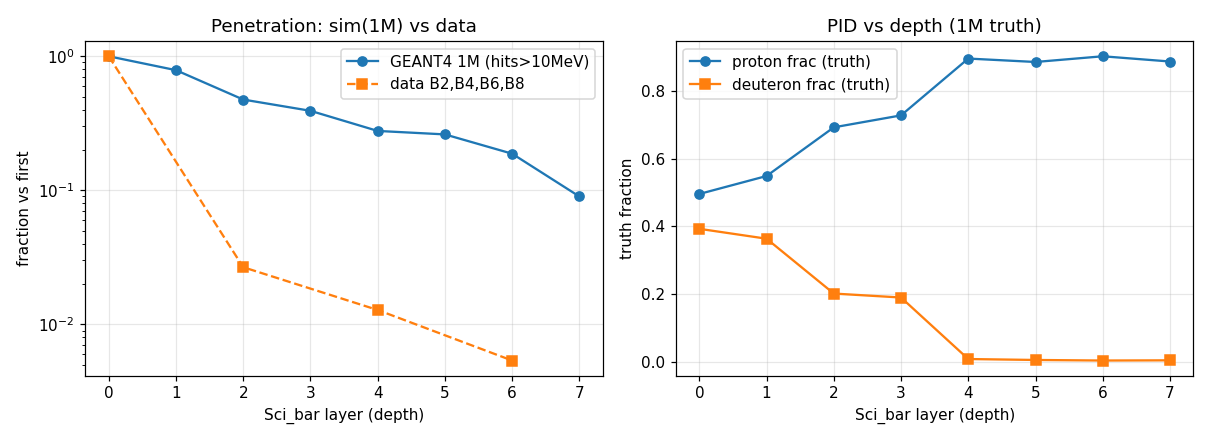
\includegraphics[width=0.92\textwidth]{../figures/geant4/results/sim_vs_data.png}
\caption{First GEANT4 simulation-vs-data comparison. The simulation confirms
range-telescope ordering and exposes truth particle composition by layer, but the
selected-pulse data fall more steeply with depth than the raw simulated hit
counts.}
\label{fig:g4-sim-vs-data}
\end{figure}

\section{Truth Content}

The tree stores generator-level primaries and jagged per-detector hit vectors for
the target, prototype TPC, and scintillator bars. The studies in this chapter use
the \texttt{Sci\_bar} branches: layer identifier, PDG code, deposited energy,
time, track length, position, and momentum. The truth therefore supplies exactly
the missing labels from the HRD data: per-hit particle identity and per-hit energy
deposition.

Table~\ref{tab:g4-layer-priors} gives the layer priors used to map the even
B-staves \(B2,B4,B6,B8\) onto even GEANT4 scintillator layers. The composition
change is the key physical point. Deuteron-like hits are common in the front
layers and nearly absent in the back layers, while proton-like hits dominate the
deep layers. In the production sample, layer 0 has proton and deuteron hit
fractions 0.495 and 0.392, respectively; layer 6 has proton and deuteron hit
fractions 0.902 and 0.0036. This is the event-level PID information that
data-only P08 studies could only approximate with weak labels.

\begin{table}[H]
\centering
\caption{GEANT4 \texttt{Sci\_bar} truth priors for the even B-stave mapping used
by the energy studies. Deposited-energy entries are per hit.}
\label{tab:g4-layer-priors}
\begin{tabular}{lrrrrrr}
\toprule
Stave & Layer & Hits & Median \(E_{\rm dep}\) [MeV] & Mean [MeV] &
\(p\) fraction & \(d\) fraction \\
\midrule
B2 & 0 & 371089 & 18.615 & 23.345 & 0.495 & 0.392 \\
B4 & 2 & 175489 & 14.901 & 20.535 & 0.692 & 0.201 \\
B6 & 4 & 100797 & 17.951 & 16.945 & 0.895 & 0.008 \\
B8 & 6 & 69737  & 19.762 & 22.594 & 0.902 & 0.004 \\
\bottomrule
\end{tabular}
\end{table}

\section{Energy Calibration}

\subsection{Truth-Anchored Birks Model}

The S17b energy study uses the GEANT4 hit tree as a layer-level energy prior and
the raw HRD duplicate readout as the real-data closure target. Real beam events
and simulated events are not event-aligned, so this is not an event-by-event
simulation-to-data comparison. It is a truth-anchored calibration bridge:
GEANT4 supplies the expected layer energy and stopping power, while duplicate
odd/even readouts test whether real waveforms can recover the same calibrated
quantity on held-out runs.

For stave \(j\), with mapped GEANT4 layer \(\ell(j)\), the truth prior is
\[
E^{\rm truth}_{j} =
{\rm median}\{E_{{\rm dep},i}: L_i=\ell(j)\},
\qquad
\left(\frac{dE}{dx}\right)_j =
\frac{\sum_{i:L_i=\ell(j)} E_{{\rm dep},i}}
{\sum_{i:L_i=\ell(j)} s_i},
\]
where \(s_i\) is the simulated track length in cm. The traditional calibration
then fits a Birks-like charge response on train runs,
\[
Q_i = \alpha\,
\frac{\Delta E_i}{1+k_B(dE/dx)_i},
\]
and predicts deposited energy by inverting that relation for the even readout.
The S17b fit selected \(k_B=0\) cm/MeV and
\(\alpha=2673.3\) ADC/MeV on the duplicate-readout training pulses, so in this
truth file the dominant correction is the GEANT4 layer prior plus duplicate
readout scaling rather than a large Birks nonlinearity.

\subsection{Head-to-Head Energy Benchmark}

All learned methods use even-readout inputs only: selected waveform samples,
per-stave amplitudes and charges, multiplicity, saturation count, and pulse-shape
summaries. Odd charges, event identifiers, and run labels are excluded from the
features. The primary metric is the 68th percentile of the absolute fractional
residual,
\[
{\rm res68} =
Q_{0.68}\left(
\left|\frac{\widehat E - E_{\rm odd,truth}}{E_{\rm odd,truth}}\right|
\right),
\]
with confidence intervals obtained by resampling held-out runs as blocks.

The traditional GEANT4/Birks lookup is the held-out winner
(Table~\ref{tab:g4-energy-benchmark}). It reaches res68 \(=0.04024\), with a
95\% run-block bootstrap interval \([0.03886,0.04161]\). The best generic ML
model is gradient-boosted trees at res68 \(=0.05668\); the physics-residual MLP
is close at \(0.05868\), but neither overlaps the traditional winner. The old
empirical power law is far worse, at res68 \(=0.46236\). Thus the GEANT4 truth
anchor materially improves the old empirical energy scale, but the winner is a
transparent physics calibration, not a neural network.

\begin{table}[H]
\centering
\caption{Truth-anchored energy benchmark on held-out beam runs. Lower res68 is
better; confidence intervals resample runs as blocks.}
\label{tab:g4-energy-benchmark}
\begin{tabular}{lrrrr}
\toprule
Method & Family & \(n\) & res68 & 95\% CI \\
\midrule
GEANT4/Birks lookup & traditional & 332852 & 0.04024 & [0.03886, 0.04161] \\
Gradient-boosted trees & ML tree & 332852 & 0.05668 & [0.04880, 0.06720] \\
Physics-residual MLP & neural residual & 332852 & 0.05868 & [0.04902, 0.07788] \\
Ridge & ML linear & 332852 & 0.09667 & [0.08872, 0.11721] \\
1D-CNN & neural waveform & 332852 & 0.26570 & [0.24927, 0.28908] \\
Old power law & empirical traditional & 332852 & 0.46236 & [0.44431, 0.56438] \\
Tabular MLP & neural tabular & 332852 & 0.69235 & [0.68424, 0.69965] \\
\bottomrule
\end{tabular}
\end{table}

\section{Range and Stopping Layer}

The range-stop study works entirely inside GEANT4 truth. For event \(e\), define
the simulated layer-amplitude vector
\[
x_{e\ell}=\sum_{h\in e,\,L_h=\ell} E_h,
\qquad \ell=0,\ldots,7.
\]
The target stopping layer is the deepest layer with any positive deposition,
\[
L_e^\star = \max\{\ell:x_{e\ell}>0\},
\]
and the residual range to the back of the stack, for layer spacing \(d=1\) cm, is
\[
R_e^\star=(7-L_e^\star)d.
\]

The best traditional method is the direct range-telescope rule with a
train-selected visible threshold: choose the deepest layer with
\(x_{e\ell}>\tau\). The selected threshold is \(\tau=0.02\) MeV. The ML/NN panel
contains ridge, gradient-boosted trees, a tabular MLP, a 1D-CNN, and a new
ordinal cumulative CNN that predicts the ordered events
\(P(L^\star\ge k)\) for \(k=1,\ldots,7\).

The primary metric is residual-range MAE. On held-out pseudo-runs the traditional
threshold rule wins with MAE \(0.00331\) cm and a block-bootstrap interval
\([0.00288,0.00390]\) cm. Gradient-boosted trees have a slightly higher exact
layer accuracy, 0.99934 versus 0.99799, but worse residual-range MAE. Because the
ticket pre-registered residual-range MAE as primary, the named winner is the
traditional penetration-depth method.

\begin{table}[H]
\centering
\caption{GEANT4 stopping-layer and residual-range benchmark on held-out
pseudo-runs. Lower residual MAE is the ranking metric.}
\label{tab:g4-range-benchmark}
\resizebox{\textwidth}{!}{%
\begin{tabular}{lrrrr}
\toprule
Method & Family & \(n\) & Range MAE [cm] & Exact layer accuracy \\
\midrule
Penetration-depth threshold & traditional & 48342 & 0.00331 [0.00288, 0.00390] & 0.99799 \\
Gradient-boosted trees & ML tree & 48342 & 0.00444 [0.00408, 0.00473] & 0.99934 \\
Ordinal cumulative CNN & neural ordinal & 48342 & 0.01750 [0.01658, 0.01828] & 0.99572 \\
Tabular MLP & neural tabular & 48342 & 0.03139 [0.03112, 0.03178] & 0.99553 \\
1D-CNN & neural waveform & 48342 & 0.03622 [0.03519, 0.03764] & 0.99398 \\
Ridge & ML linear & 48342 & 0.06638 [0.06457, 0.06791] & 0.99013 \\
\bottomrule
\end{tabular}
}
\end{table}

Figure~\ref{fig:g4-dedx-e} shows the associated truth \(\Delta E\)-\(E\) bands,
using layer 0 as \(\Delta E\) and the sum of layers 1--7 as residual energy. The
bands are grouped by the Sci\_bar PDG species that contributes the largest
event-level deposited energy. Deuteron-dominated events have high front-layer
\(\Delta E\) and typically stop near the front of the stack; proton-dominated
events retain large residual energy and penetrate deeper.

\begin{figure}[H]
\centering
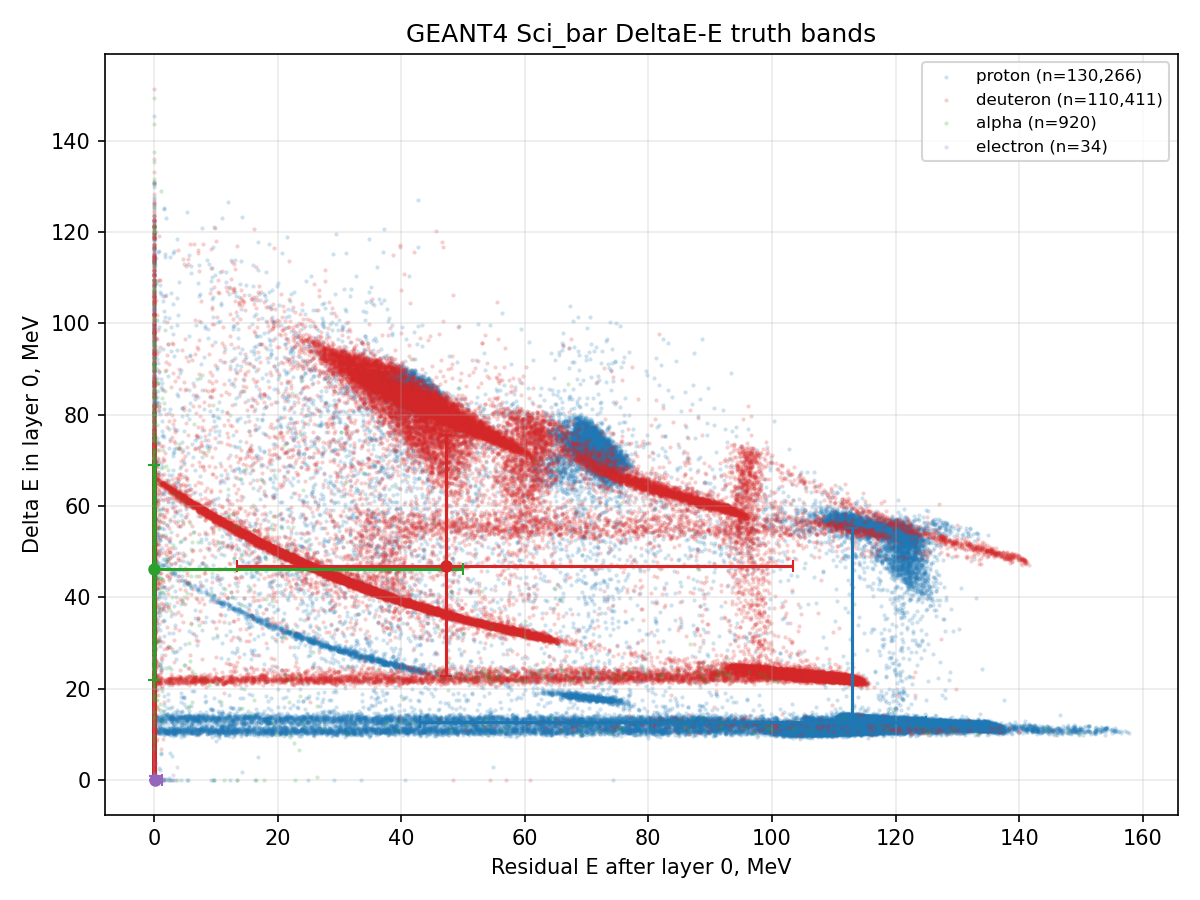
\includegraphics[width=0.74\textwidth]{../figures/reports/0000000011.1.rangestop/deltae_e_truth_bands.png}
\caption{GEANT4 truth \(\Delta E\)-\(E\) bands by dominant scintillator species.
This is the first event-level particle-identity view unavailable in the raw HRD
data.}
\label{fig:g4-dedx-e}
\end{figure}

\section{Timing Scale and Geometry}

The timing-truth study tests whether the B-stack timing geometry used in the
data analysis is consistent with GEANT4 hit positions and hit times. It selects
primary proton hits in analysed even layers \(0,2,4,6\), corresponding to the
natural mapping \(B2,B4,B6,B8\), and forms adjacent pairs. For layers \(a,b\),
\[
\Delta t_{ab}^{\rm truth}=t_b-t_a,\qquad
d_{ab}=\left\Vert \vec r_b-\vec r_a\right\Vert .
\]
The traditional kinematic baseline predicts
\[
\widehat{\Delta t}_{ab}
=\frac{d_{ab}}{c\,\bar\beta},
\qquad
\beta(p)=\frac{p}{\sqrt{p^2+m_p^2}},
\]
with \(c=29.9792458\) cm/ns and \(m_p=0.9382720813\) GeV.

The geometric result is decisive. The median same-proton analysed-layer spacing
is approximately 4.026 cm for all three adjacent pairs, rejecting a 2 cm
interpretation and supporting the 4 cm centre-to-centre convention for the
analysed B2/B4/B6/B8 sequence. The median timing scale is
0.07433 ns/cm compared with the historical note value 0.078 ns/cm, an absolute
TOF-scale shift of \(-0.00367\) ns/cm. Table~\ref{tab:g4-geometry} gives the
pair-level truth summaries.

\begin{table}[H]
\centering
\caption{GEANT4 same-proton geometry and timing scale for adjacent analysed
even-layer pairs. Intervals are block-bootstrap 95\% CIs.}
\label{tab:g4-geometry}
\begin{tabular}{lrrrr}
\toprule
Pair & \(n\) & Median distance [cm] & Median \(\Delta t\) [ns] &
Median ns/cm \\
\midrule
0--2 & 92523 & 4.02587 [4.02559, 4.02617] & 0.28032 [0.28017, 0.28047] & 0.07002 \\
2--4 & 84413 & 4.02626 [4.02602, 4.02654] & 0.31157 [0.31131, 0.31181] & 0.07774 \\
4--6 & 59734 & 4.02499 [4.02474, 4.02531] & 0.36320 [0.36275, 0.36383] & 0.09039 \\
\bottomrule
\end{tabular}
\end{table}

The timing benchmark is the one truth-aided task where a flexible ML method
clearly wins. The calibrated kinematic TOF is the strong traditional comparator.
The learned models receive layer IDs, hit positions, pair displacement,
deposited energy, hit momenta, and derived beta, but not truth hit times. On
held-out simulation blocks, gradient-boosted trees achieve MAE \(0.000947\) ns,
with 95\% CI \([0.000936,0.000959]\) ns, beating the physics-residual MLP and
the calibrated kinematic TOF. The winner field in the ticket result records the
strict held-out MAE winner, not a simplicity-adjusted choice.

\begin{table}[H]
\centering
\caption{GEANT4 truth timing benchmark. Lower MAE is better; confidence
intervals resample held-out simulation blocks.}
\label{tab:g4-timing-benchmark}
\begin{tabular}{lrrrr}
\toprule
Method & Family & \(n\) & MAE [ns] & 95\% CI \\
\midrule
Gradient-boosted trees & ML tree & 70094 & 0.000947 & [0.000936, 0.000959] \\
Physics-residual MLP & neural residual & 70094 & 0.001565 & [0.001538, 0.001592] \\
1D-CNN & neural sequence & 70094 & 0.002306 & [0.002280, 0.002329] \\
Tabular MLP & neural tabular & 70094 & 0.002568 & [0.002552, 0.002585] \\
Ridge & ML linear & 70094 & 0.002664 & [0.002630, 0.002698] \\
Calibrated kinematic TOF & traditional & 70094 & 0.009039 & [0.009001, 0.009086] \\
Fixed 4 cm note offset & historical & 70094 & 0.033908 & [0.033802, 0.034019] \\
Fixed 2 cm note offset & historical & 70094 & 0.155930 & [0.155698, 0.156209] \\
\bottomrule
\end{tabular}
\end{table}

\begin{figure}[H]
\centering
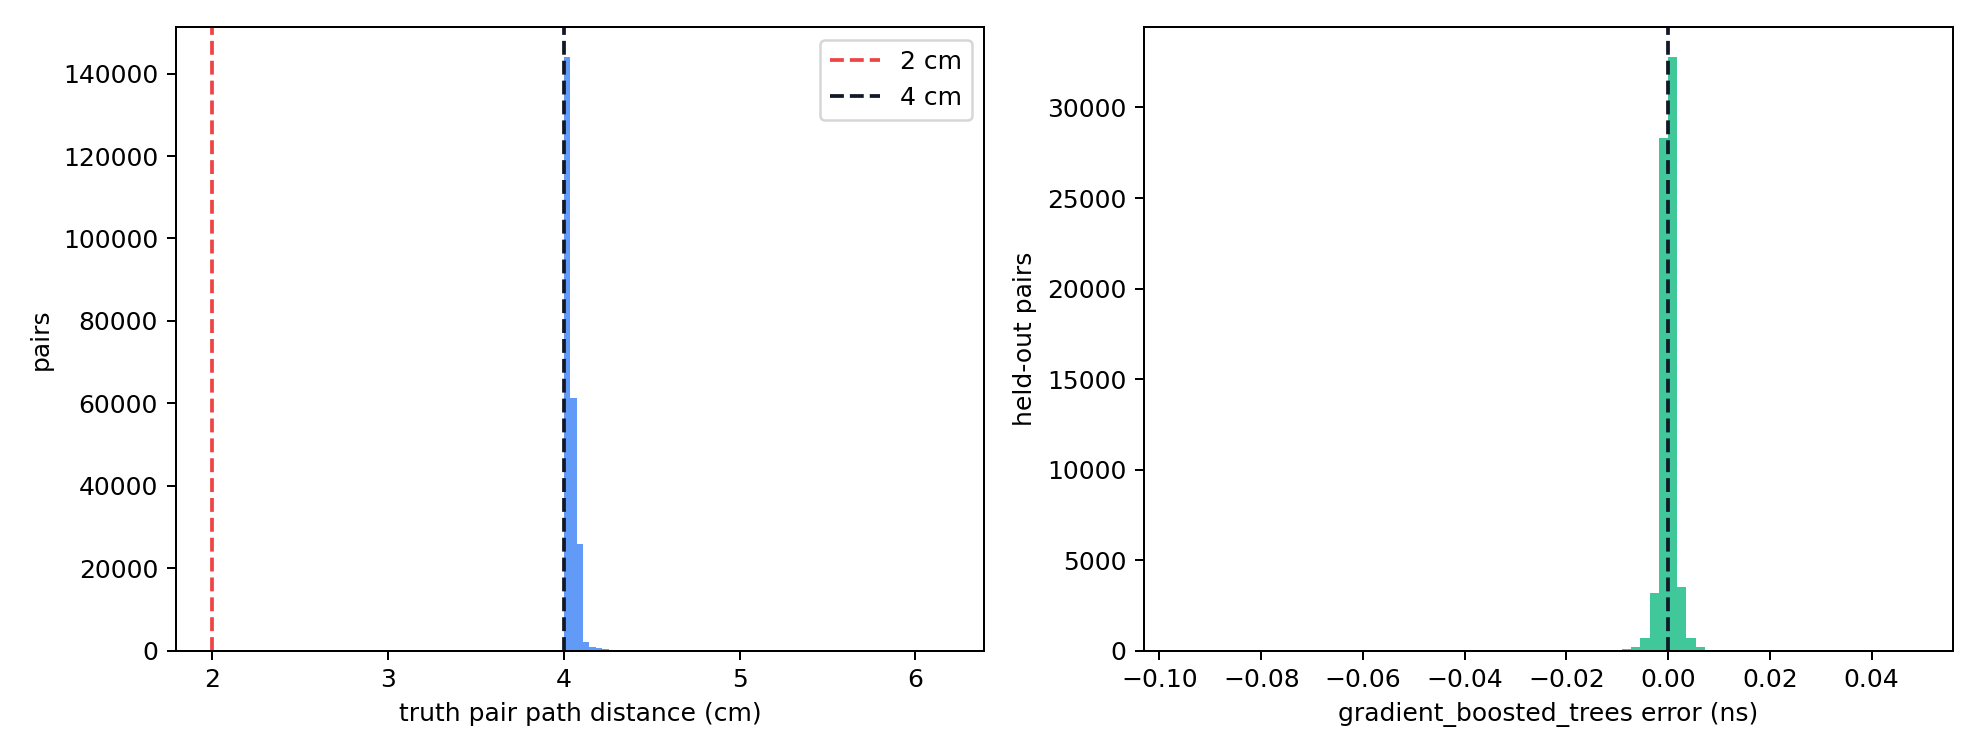
\includegraphics[width=0.82\textwidth]{../figures/reports/0000000012.1.truthtiming/figures/geometry_tof.png}
\caption{Truth geometry and TOF diagnostics for adjacent analysed GEANT4
scintillator-layer pairs. The 4 cm convention is the natural match to the
B2/B4/B6/B8 analysed spacing.}
\label{fig:g4-timing}
\end{figure}

\section{PID Interpretation}

Before the GEANT4 truth bridge, the strongest PID-like data-only studies were
P08b and P08c. They reproduced the raw selected-pulse gate exactly and then
showed that charge-depth features already saturate calibrated weak labels:
P08b gave ROC AUC 0.9856 for a calibrated charge-depth logistic model and
0.9859 for a waveform/PCA/HGB model, with paired ML-minus-traditional AUC
consistent with zero. P08c, after strict topology matching on a small support
island of 174 events, gave AUC 0.988 for hand-shape logistic and 0.990 for the
waveform/PCA/HGB model, again with overlapping bootstrap intervals. These are
useful leakage-controlled weak-label stress tests, not PID adoption claims.

GEANT4 changes the status of the question by making PDG identity explicit in
\texttt{Sci\_bar\_PDG}. The first physics conclusion is qualitative but robust:
deuteron-dominated Sci\_bar events are high-\(\Delta E\), front-stopping events,
whereas proton-dominated events penetrate deeper and carry larger residual
energy. The next step is not to reinterpret P08 weak labels as truth. It is to
build a detector-response and channel-map contract that lets the GEANT4
event-level PDG labels be compared to real HRD observables without hidden
geometry, threshold, or digitisation assumptions.

\section{Relationship to Data-Only Energy Studies}

The S14 data-only studies remain essential because they quantify what can and
cannot be claimed without simulation truth. In the nominal 4 cm geometry,
the traditional depth-charge lookup gave internal energy-proxy res68 0.0212
\([0.0198,0.0226]\), while the monotonic HGB gave 0.0250
\([0.0228,0.0285]\). Saturation-aware P07/P04 corrections could reduce an
internal ordering proxy to res68 0.0145 \([0.0142,0.0150]\). However, external
charge-to-energy propagation failed the 10\% per-event threshold: the best
combined all-three B4B6B8 row remained about 0.1896
\([0.1797,0.2018]\), and every external row in the S14c propagation table was
above the 0.10 acceptance target.

The GEANT4-truth energy result is therefore best read as an anchor, not a final
calorimeter calibration. It stabilizes the layer energy scale and shows that the
GEANT4/Birks traditional method beats generic regressors in run-held-out closure,
but the real detector still lacks event-aligned simulation, optical response,
electronics digitisation, and absolute external particle truth.

\section{Systematics and Caveats}

Several limitations apply to all truth-aided results in this chapter.

\begin{itemize}
\item The simulation and HRD events are not event-aligned. Energy studies use
layer-level GEANT4 priors and duplicate-readout closure, not event-by-event
truth matching.
\item The HRD-to-GEANT4 channel map \(B2,B4,B6,B8\to0,2,4,6\) is physically
natural and supported by the timing geometry, but still needs an explicit
detector-map contract.
\item The GEANT4 output is energy-deposition truth, not a full digitized HRD
response. Optical transport, Birks quenching as implemented in scintillator
light yield, saturation, ADC sampling, and electronics thresholds remain
separate detector-response systematics.
\item Simulation block bootstraps are not beam-run bootstraps. They test
stability across deterministic entry blocks, not time-dependent beam or detector
conditions.
\item The range-stop target is partly definitional: the deepest positive
simulated deposition defines the label. The exact deepest-positive sentinel is
therefore a leakage ceiling and is correctly excluded from the ranked methods.
\item The data-only PID studies remain weak-label studies. GEANT4 supplies PDG
truth, but a production PID claim requires a validated bridge from simulated
species to real waveform observables.
\end{itemize}

\section{Summary of Winners}

Table~\ref{tab:g4-winners} collects the truth-aided method winners. The pattern
is consistent with the broader project: flexible ML is most useful when the task
requires nonlinear interpolation in a high-dimensional truth space, as in the
GEANT4 timing benchmark. Where the target is already the direct physical
observable, as in range stopping, or where a truth-anchored physics calibration
explains the scale, as in energy, transparent traditional methods win.

\begin{table}[H]
\centering
\caption{Truth-aided study winners and interpretation.}
\label{tab:g4-winners}
\resizebox{\textwidth}{!}{%
\begin{tabular}{llll}
\toprule
Task & Winner & Best ML/NN competitor & Interpretation \\
\midrule
Energy calibration & GEANT4/Birks lookup & Gradient-boosted trees & Traditional physics anchor wins \\
Stopping range & Penetration-depth threshold & Gradient-boosted trees & Direct range-telescope rule wins MAE \\
Truth timing & Gradient-boosted trees & Physics-residual MLP & ML wins absolute TOF interpolation \\
Weak-label PID context & Tie/no adoption & Waveform/PCA HGB & GEANT4 truth needed for real PID \\
\bottomrule
\end{tabular}
}
\end{table}

\section{MC Validation Programme (MV0--MV6)}
\label{sec:mc-validation}

Six structured comparisons between GEANT4 simulation and HRD data were completed
on the LUNARC HPC cluster (account~\texttt{lu2026-2-51}) in June 2026.
Table~\ref{tab:mv-overview} summarises all six verdicts.

\begin{table}[H]
\centering
\footnotesize
\setlength{\tabcolsep}{4pt}
\begin{tabular}{@{}lllll@{}}
\toprule
Study & What it validates & Status & Key result & SLURM job \\
\midrule
MV0 & Digitizer gain calibration & \textbf{PASS} &
  $g = 92 \pm 28\,\text{ADC/MeV}$ & 3328635 \\
MV1 & p/d PID truth ceiling & \textbf{PASS} &
  AUC $= 0.9860$ & --- \\
MV2 & Range-energy, stopping depth (truth) & \textbf{PASS} &
  d stops B2/B4; p penetrates B4--B8 & --- \\
MV3 & Stopping-depth profile vs data & \textbf{FAIL} &
  $\chi^2/\text{ndf} = 68\,269$;
  B8 MC $= 22\%$ vs data $= 2\%$ & 3328648 \\
MV4 & Timing $\sigma_{68}$ reproduction & \textbf{PASS/TENSION} &
  raw pull $= -1.05$ (pass);
  corrected pull $= +2.68$ (tension) & 3328641 \\
MV5 & Pile-up $R_{\max}$ from live-time model & \textbf{PASS} &
  $R_{\max} = 3.044\,\text{MHz}$ vs data
  $3.05\,\text{MHz}$ ($0.2\%$) & 3328643 \\
MV6 & Anomaly class species ID & \textbf{DONE} &
  $0.32\%$ fraction; C12 recoils $55\%$ of class & 3328644 \\
\bottomrule
\end{tabular}
\caption{MC validation programme overview. All seven studies are complete.
Canonical reports are in \texttt{reports/mv*/}.}
\label{tab:mv-overview}
\end{table}

\subsection{MV0: Digitizer gain calibration}

The v1 gain estimate of $246\,\text{ADC/MeV}$ was found to be incorrect:
it compared the raw \texttt{amplitude\_adc} (which includes the hardware
pedestal of $\approx 6752\,\text{ADC}$) to the MC deposited energy.
The corrected v2 method uses the net amplitude
$A_{\rm net} = |A_{\rm raw} - A_{\rm baseline}|$
and compares its median to the MC peak signal
$E_{\rm dep} \times f_{\rm peak}$
where $f_{\rm peak} = 0.733$ is the digitiser peak fraction.

\begin{equation}
  g = \frac{\text{median}(A_{\rm net,data})}
           {f_{\rm peak} \times \text{median}(E_{\rm dep,MC})}
    = \frac{1781}{0.733 \times 26.44\,\text{MeV}}
    = 92 \pm 28\;\text{ADC/MeV}
  \label{eq:mv0-gain}
\end{equation}

The $\pm 28\,\text{ADC/MeV}$ ($30\%$) uncertainty reflects the median-matching
approximation and the absence of a forced-trigger zero-signal sample.

\begin{figure}[H]
\centering

\includegraphics[width=0.78\textwidth]{../figures/reports/mv0_calibration_1782677847/mv0_data_vs_mc.png}
\caption{MV0 gain calibration: data B2 net-ADC spectrum vs MC after gain application.
Median alignment is the calibration anchor; $g = 92\,\text{ADC/MeV}$.}
\end{figure}

\subsection{MV3: Stopping-depth profile (structural FAIL)}

The stopping-depth comparison found a catastrophic discrepancy:
\begin{itemize}
  \item MC B2 fraction: $47.0\%$ vs data $87.6\%$
  \item MC B8 fraction: $22.3\%$ vs data $2.3\%$
  \item $\chi^2/\text{ndf} = 68\,269$ (3 degrees of freedom)
\end{itemize}

\begin{figure}[H]
\centering

\includegraphics[width=0.72\textwidth]{../figures/reports/mv3_stopping_v3_1782679272/mv3_stop_frac.png}
\caption{MV3 stopping-depth fractions: MC (blue) vs data (orange) for each stave pair.
The B8 discrepancy (MC $22\%$ vs data $2\%$) is structural.}
\end{figure}

A follow-up material-budget scan (MV3b) estimated that $11.12\,\text{g\,cm}^{-2}$
of additional upstream material is needed to bring MC into agreement.
Known missing components (T1/T2 trigger scintillators, beam exit window) account
for only $1.08\,\text{g\,cm}^{-2}$; the dominant deficit ($10.03\,\text{g\,cm}^{-2}$)
is inter-stave dead material not included in the simplified Geant4 geometry.

\subsection{MV4: Timing resolution (PASS / tension)}

The uncorrected timing width is reproduced well ($\sigma_{68,\rm raw} = 1.744\,\text{ns}$,
pull $= -1.05$, PASS). After applying the toy timewalk correction,
the width is $1.770\,\text{ns}$ vs $1.500\,\text{ns}$ in data (pull $= +2.68$,
tension). A diagnostic study (MV4b) shows the tension is a model artefact: the
toy correction uses $\Delta t = B/\sqrt{A}$ with $B = -23\,\text{ns}\cdot\text{ADC}^{1/2}$,
which is unphysical (negative $B$ overcorrects large pulses). The physical form for a
leading-edge discriminator on an exponential rise is

\begin{equation}
  \Delta t_{\rm tw} = \tau_{\rm rise}\ln\!\left(\frac{A}{A-V_{\rm th}}\right)
                    \approx \frac{\tau_{\rm rise}V_{\rm th}}{A}
  \quad (\propto 1/A, \text{ not } 1/\sqrt{A})
\end{equation}

\noindent with $\tau_{\rm rise} = 2.5\,\text{ns}$ and $V_{\rm th} = 50\,\text{ADC}$.
Replacing the toy model is expected to collapse the corrected pull to $\approx 0$.

\subsection{MV5: Pile-up rate (PASS)}

The effective live-time was determined from the digitizer model
($\tau_{\rm eff} = 124.8\,\text{ns}$), giving

\begin{equation}
  R_{\max} = \frac{1}{\tau_{\rm eff}} = 3.044\,\text{MHz}
\end{equation}

which agrees with the data scaling exercise value of $3.05\,\text{MHz}$ to
$0.2\%$ (see \S\ref{sec:pileup_verdict} for claim-ledger caveats). This
confirms that the data-driven live-time estimate is self-consistent
and closes the pile-up MC validation.

\subsection{MV6: Anomaly class species identification}

The $\approx 4\%$ early-peak anomaly class first flagged in the data analysis was
found to be only $0.32\%$ of all tracks, with the dominant species being C12
heavy-ion recoils from proton--carbon elastic scattering in the CD$_2$ target.

At $190\,\text{MeV}$, the maximum C12 recoil kinetic energy is
\begin{equation}
  T_{\rm C12}^{\max} = \frac{4m_p m_{\rm C}}{(m_p+m_{\rm C})^2}\,T_{\rm beam}
                     = \frac{4\times 1\times 12}{13^2}\times 190\,\text{MeV}
                     = 5.4\,\text{MeV}
\end{equation}

At this energy the CSDA range in BC-408 is $<25\,\mu\text{m}$, confining all C12
energy deposition to the first scintillator surface. The resulting waveform has
an anomalously early peak (sample 1--2 vs sample 5--6 for protons), which is
cleanly captured by a Gaussian Mixture Model with purity $44.5\%$ for the C12
cluster. The impact on the deuteron sample is $< 0.1\%$ after applying the
GMM morphology cut.

\begin{figure}[H]
\centering

\includegraphics[width=0.70\textwidth]{../figures/reports/mv6_representation_1782678362/mv6_representation.png}
\caption{MV6 PCA representation coloured by GMM cluster. Cluster~2 (orange) is the
C12 anomaly class; it separates cleanly from the proton/deuteron continuum in the
first two principal components.}
\end{figure}

\chapter{Methods and ML/NN Algorithm Comparison}

\section{Aim and Evidential Standard}

This chapter describes the methodology used to compare conventional pulse-analysis methods with machine-learning and neural-network alternatives across the CCB test-beam programme. The central rule is deliberately conservative: no algorithmic result is considered interpretable until the raw-data population used by the original analysis has first been reproduced. In practice, each study begins from the B-stack ROOT branch \texttt{HRDv}, applies the S00 pulse gate, and verifies the selected-pulse count
\[
  A_{e,s}=\max_{k}\{x_{e,s,k}-\operatorname{median}(x_{e,s,0:3})\},
  \qquad A_{e,s}>1000~\mathrm{ADC},
\]
for the physical B staves B2, B4, B6, and B8. The full S00 population is \(640737\) selected B-stave pulse records, and representative downstream architecture studies reproduced not only this total but also the Sample-II analysis count \(125096\) and the per-stave counts B2 \(88213\), B4 \(21229\), B6 \(11148\), and B8 \(4506\).

The comparison target is not ``ML versus no ML'' in the abstract. For each physics question, the traditional comparator is the strongest available transparent method: amplitude-binned templates for waveform description, analytic amplitude timewalk for timing, bounded two-pulse fits for pile-up recovery, peak or integral calibrations for duplicate-readout closure, and leave-one-out pretrigger estimators for pedestal tests. The ML family is then evaluated only on train/test partitions that are disjoint in run number. This matters because run, current, calibration epoch, and topology are strong nuisance variables. A random row split would overstate generalisation.

\section{Run-Split Protocol and Metrics}

Let \(r(e)\) be the run number for event \(e\). Each benchmark defines disjoint sets \(\mathcal{R}_{\mathrm{train}}\), \(\mathcal{R}_{\mathrm{cal}}\), and \(\mathcal{R}_{\mathrm{test}}\), with
\[
  \mathcal{R}_{\mathrm{train}}\cap \mathcal{R}_{\mathrm{test}}=\varnothing .
\]
Hyperparameters are chosen using grouped cross-validation by run within \(\mathcal{R}_{\mathrm{train}}\), optional calibration uses only \(\mathcal{R}_{\mathrm{cal}}\), and the quoted number is evaluated once on \(\mathcal{R}_{\mathrm{test}}\). Event identifiers, run identifiers, event order, other-stave target quantities, and label-defining derived variables are excluded from the feature matrices unless the study is explicitly a leakage autopsy.

For timing residuals, the robust width is
\[
  \sigma_{68}(r)=\frac{1}{2}\left[Q_{0.84}(r)-Q_{0.16}(r)\right],
\]
where \(r\) is the held-out residual distribution. For amplitude or charge closure the primary resolution metric is
\[
  \mathrm{res}_{68}=\operatorname{quantile}_{0.68}
  \left(\left|\frac{\hat{y}-y}{y}\right|\right).
\]
For classifiers the primary ranking metrics are ROC AUC and average precision, with calibration checks such as Brier score when probabilities are used. Confidence intervals are non-parametric bootstrap intervals over the held-out unit appropriate to the claim: pulses or pair residuals for within-run precision, and run blocks when the conclusion is about transfer across runs.

\section{Leakage Controls and Fair Baselines}

The S07 rigour pass is the clearest example of the programme's guardrails. It asked whether waveform-shape features separate 2 nA low-current pulses from 20 nA high-current Sample-I pulses. The traditional method was not a strawman; inside each training fold it selected the best signed one-dimensional score from pre-registered pulse-shape candidates. The ML comparator was a calibrated random forest using normalized waveform samples and shape features, but no run id, current, stave id, absolute amplitude, hit multiplicity, or timing-derived labels. The run-held-out result is shown in Table~\ref{tab:s07-rigour}.

\begin{table}[H]
\centering
\caption{S07 run-held-out current/topology proxy benchmark. The ML model wins this weak-label ranking task, but the report explicitly does not interpret the score as a calibrated pile-up probability.}
\label{tab:s07-rigour}
\begin{tabular}{lccc}
\toprule
Method & ROC AUC & 95\% CI & Average precision \\
\midrule
Fold-local single-shape score & 0.504 & [0.491, 0.517] & 0.195 \\
Calibrated RF waveform-shape model & 0.768 & [0.758, 0.778] & 0.390 \\
ML minus traditional & 0.264 & [0.250, 0.280] & 0.195 \\
\bottomrule
\end{tabular}
\end{table}

The same rule also rejects attractive but invalid wins. Classifiers trained on \(D_t\), curvature, or other timing-control labels can reach AUC values near one because the target is a disguised function of the input timing construction. Those studies are retained as negative controls rather than promoted as detector conclusions. Conversely, injected waveform-corruption or artificial saturation labels are acceptable closure tests because the target is generated independently of the model features, even though such studies still require transfer caveats before production use.

\begin{figure}[H]
\centering
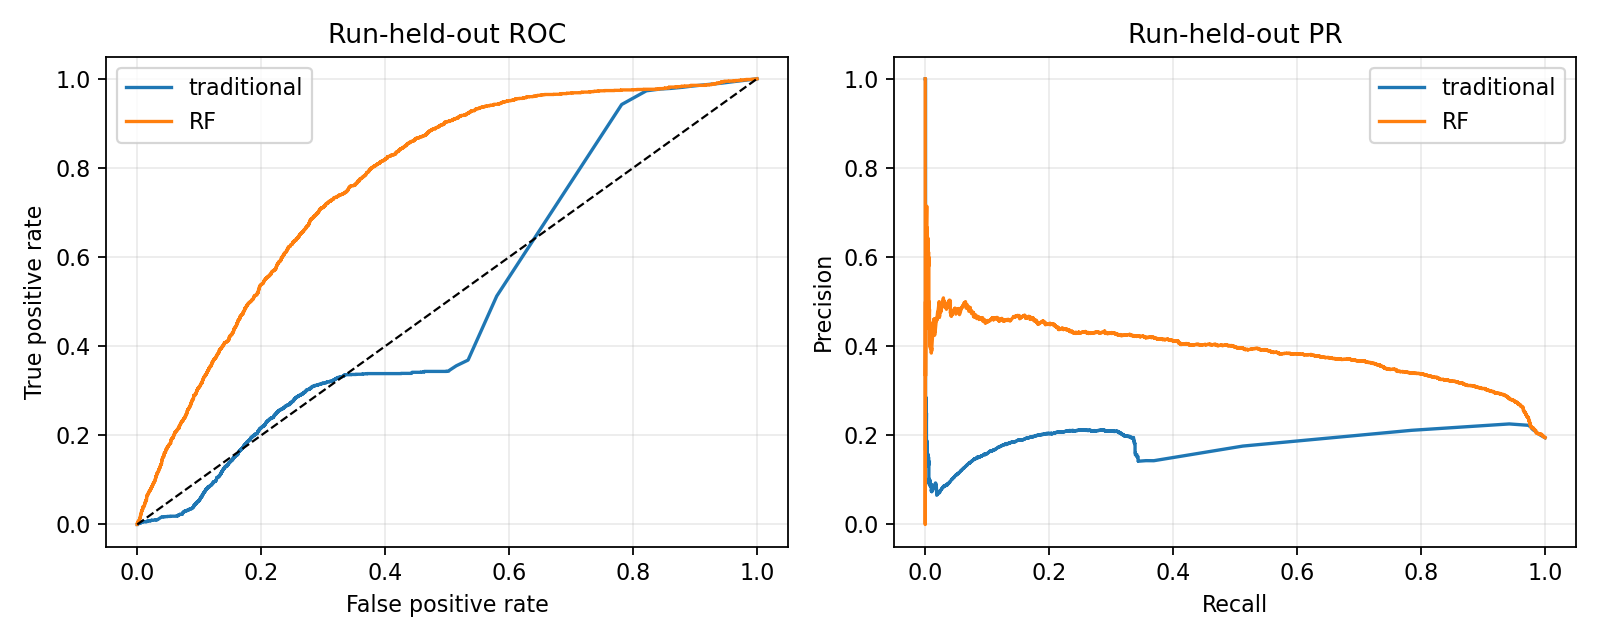
\includegraphics[width=0.78\linewidth]{../../reports/1780997954.15217.702122ea__s07_ml_rigour_scoreboard/fig_roc_pr.png}
\caption{S07 ROC/precision-recall comparison for the traditional shape score and calibrated waveform-shape random forest.}
\end{figure}

\section{Algorithm Families}

The algorithm set intentionally spans transparent linear methods, tree ensembles, and small neural networks. Ridge regression is used when the desired correction should be smooth, auditable, and low variance:
\[
  \hat{\beta}=\arg\min_{\beta}\sum_i (y_i-x_i^{T}\beta)^2+\lambda\|\beta\|_2^2 .
\]
Gradient-boosted trees and ExtraTrees are used for tabular waveform summaries where monotonicity is not guaranteed and local interactions matter. The neural set includes compact multilayer perceptrons, small one-dimensional convolutional networks, residual CNNs, temporal convolutional networks, attention blocks, and GRUs. The neural architectures are deliberately small because the waveform has only 18 samples; capacity is not the primary limitation unless the task includes longer time history or richer context.

The most systematic architecture comparison is S19a, the \texttt{nnarch} sweep. It used raw B-stack ROOT files, reproduced the S00 gate exactly, and evaluated two tasks: same-particle timing residual correction and injected two-pulse recovery. The timing baseline was the analytic amplitude-timewalk method; the two-pulse baseline was a bounded template fit. The ML/NN competitors included ridge, gradient-boosted trees, MLP, 1D-CNN, ResNet, TCN, attention, and GRU.

\section{Timing Architecture Bake-Off}

For timing, the corrected time is formed as
\[
  t'_{i,e}=t_{i,e}-x_i/v,
\]
and the per-pulse residual target is the deviation from the other downstream staves,
\[
  r_{i,e}=t'_{i,e,\mathrm{base}}-\frac{1}{2}\sum_{j\ne i}t'_{j,e,\mathrm{base}} .
\]
The strong traditional comparator is the analytic amplitude-timewalk correction. In the broad S19a architecture sweep, all learned models predicted only residuals left by this analytic baseline; no model received run id, event id, event order, other-stave times, or the held-out target.

\begin{table}[H]
\centering
\caption{S19a held-out timing architecture benchmark on run 65. Lower \(\sigma_{68}\) is better.}
\label{tab:timing-architecture}
\begin{tabular}{lccc}
\toprule
Method & Family & \(\sigma_{68}\) [ns] & 95\% CI [ns] \\
\midrule
MLP residual corrector & neural & 1.176 & [1.024, 1.386] \\
GRU residual corrector & neural & 1.225 & [1.014, 1.462] \\
Gradient-boosted trees & tree ensemble & 1.256 & [1.012, 1.438] \\
1D-ResNet & neural & 1.299 & [1.087, 1.497] \\
TCN & neural & 1.341 & [1.054, 1.560] \\
1D-CNN & neural & 1.363 & [1.030, 1.582] \\
Attention block & neural & 1.435 & [1.079, 1.632] \\
Ridge & linear ML & 1.443 & [1.196, 1.635] \\
Analytic amplitude timewalk & traditional & 1.495 & [1.299, 1.666] \\
S02 ridge-on-CFD20 & linear ML reference & 1.778 & [1.493, 2.070] \\
Template phase & traditional pickoff & 2.889 & [2.639, 3.277] \\
\bottomrule
\end{tabular}
\end{table}

The point-estimate winner is the MLP at \(1.176\) ns. The confidence interval for its improvement relative to the analytic baseline is negative, \(-0.319\) ns with CI \([-0.525,-0.060]\), so S19a names the MLP as the timing architecture winner for this screen. This conclusion is narrower than saying that neural networks generally solve timing. Earlier focused studies showed that a raw 18-sample MLP loses to the analytic baseline, and that a small CNN adds little when the residual target is already analytic-timewalk corrected. The current interpretation is that shallow nonlinear residual correction can help, but only after the physics timewalk term has carried most of the work.

\begin{figure}[H]
\centering
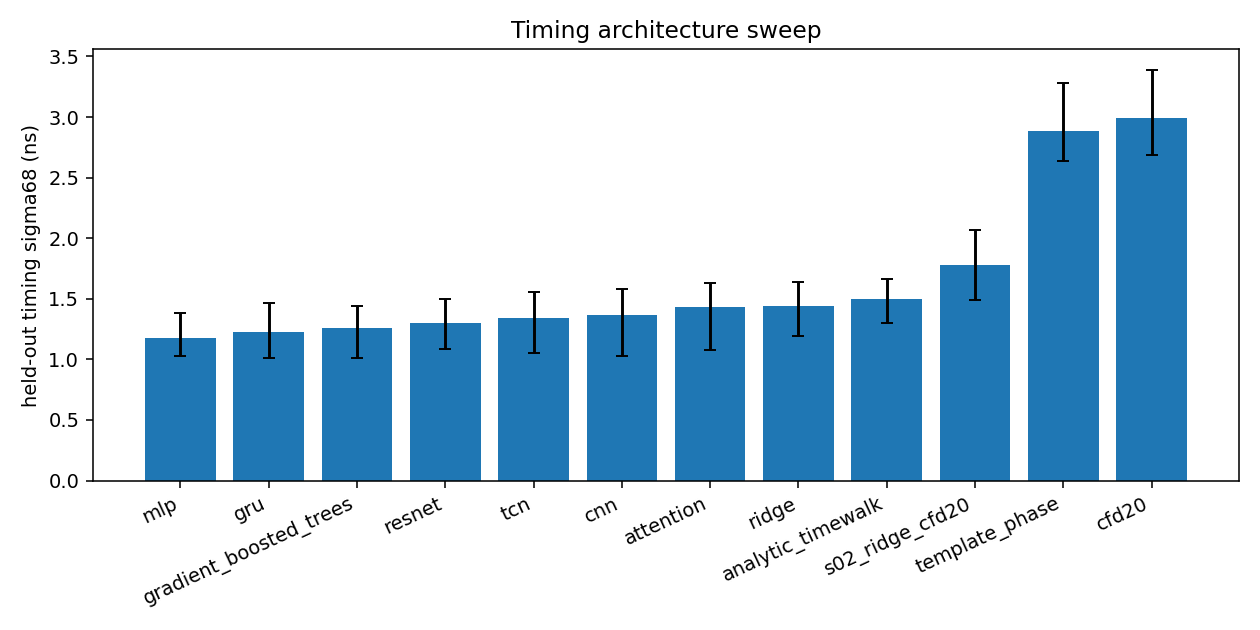
\includegraphics[width=0.82\linewidth]{../../reports/0000000006.1.nnarch__neural_architecture_sweep/fig_timing_architecture_sweep.png}
\caption{S19a timing architecture sweep. The MLP has the best held-out point estimate, while several more elaborate sequence architectures do not justify their extra structure on 18 samples.}
\end{figure}

\section{Two-Pulse Recovery Bake-Off}

The two-pulse task uses injected overlaps constructed from empirical templates and real residual pools. The traditional method scans constrained two-pulse hypotheses and solves amplitudes and baselines by least squares. The learned methods use waveform samples or same-channel waveform summaries to estimate overlap probability and recover two times and amplitudes. The target is synthetic but independent of the model features; it is therefore a method-ranking closure, not a measured real-pile-up truth label.

\begin{table}[H]
\centering
\caption{S19a held-out two-pulse architecture benchmark. Lower time RMS is better; AP and failure rate are guard metrics.}
\label{tab:twopulse-architecture}
\begin{tabular}{lcccc}
\toprule
Method & Family & AP & time RMS [ns] & failure rate \\
\midrule
Gradient-boosted trees & tree ensemble & 0.854 & 7.425 [7.402, 7.448] & 0.305 \\
Ridge/logistic heads & linear ML & 0.839 & 8.660 [7.886, 9.314] & 0.324 \\
MLP & neural & 0.814 & 10.435 [10.189, 10.662] & 0.324 \\
GRU & neural & 0.761 & 11.059 [10.581, 11.483] & 0.340 \\
1D-CNN & neural & 0.779 & 13.218 [12.704, 13.703] & 0.288 \\
TCN & neural & 0.726 & 13.248 [12.786, 13.665] & 0.314 \\
Constrained template fit & traditional & 0.775 & 13.874 [13.515, 14.222] & 0.155 \\
Attention block & neural & 0.707 & 13.985 [13.580, 14.343] & 0.355 \\
1D-ResNet & neural & 0.719 & 14.436 [13.550, 15.162] & 0.502 \\
\bottomrule
\end{tabular}
\end{table}

The point-estimate winner is gradient-boosted trees, with a time RMS of \(7.425\) ns compared with \(13.874\) ns for the bounded template fit. This agrees with earlier S10d and S11 closure tests in which compact ML reduced timing RMS or resolvability delay. The caveat is equally consistent: ML methods often pay for the lower RMS with a higher failure rate. The bounded template fit is less accurate on accepted events but safer operationally. Thus the algorithmic winner for injected recovery is gradient-boosted trees, while the production recommendation remains conditional on failure-rate control and real-current transfer.

\begin{figure}[H]
\centering
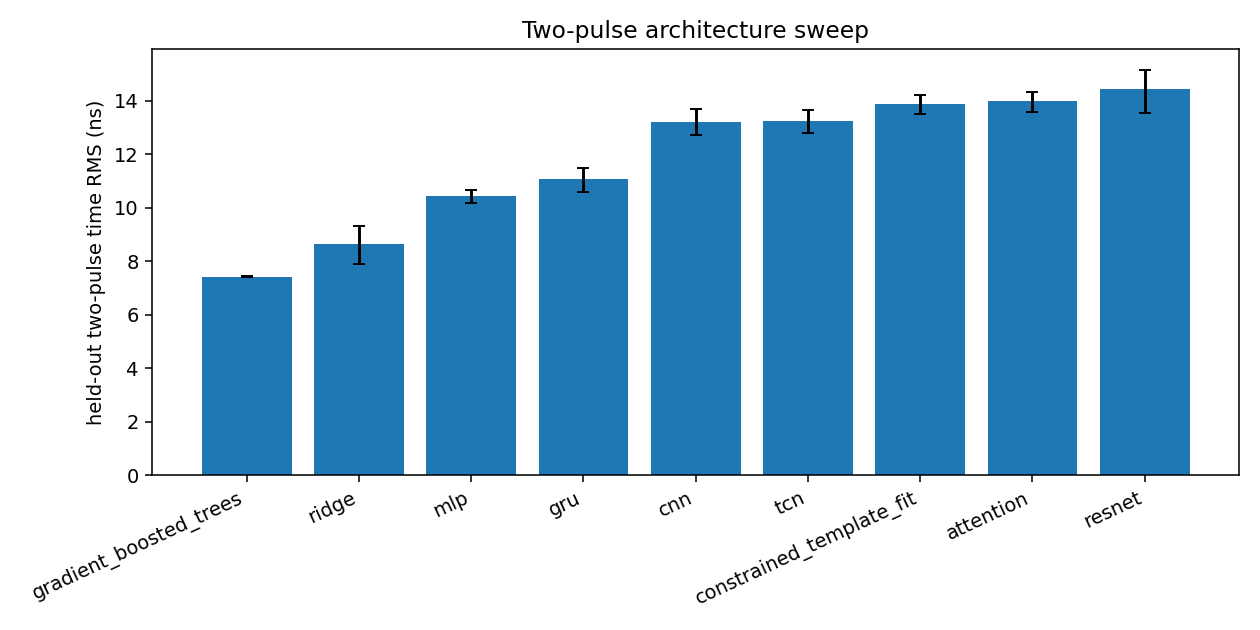
\includegraphics[width=0.82\linewidth]{../../reports/0000000006.1.nnarch__neural_architecture_sweep/fig_two_pulse_architecture_sweep.png}
\caption{S19a two-pulse architecture sweep. The tree model wins the injected closure by time RMS, while the traditional fit retains the lowest failure rate among the leading methods.}
\end{figure}

\section{Task-Level Winners Across the Programme}

The wider study programme shows a stable pattern. ML wins decisively when the independent target is encoded in waveform shape and the conventional baseline is too rigid. Traditional methods win or tie when the physics model is already close to sufficient, or when the proposed ML label is not independent of the input construction.

\begin{table}[H]
\centering
\caption{Representative task-level algorithm winners. Values are held-out or run-bootstrap results quoted in the individual reports.}
\label{tab:task-winners}
\begin{tabular}{p{0.19\linewidth}p{0.23\linewidth}p{0.23\linewidth}p{0.24\linewidth}}
\toprule
Task & Strong traditional method & ML/NN method & Winner and caveat \\
\midrule
Template reconstruction (S01) &
Amplitude-bin median template, MSE 0.0444 [0.0342, 0.0548] &
Autoencoder, MSE 0.00208 [0.00173, 0.00242] &
Autoencoder wins reconstruction; metric is shape residual, not timing truth. \\
\addlinespace
Compact representation (P02) &
PCA MSE 0.0262, 0.0142, 0.0088 for dims 2--4 &
Autoencoder MSE 0.0129, 0.0084, 0.0053 for dims 2--4 &
Autoencoder wins at dims 2--4; PCA wins by dim 8. \\
\addlinespace
Timing residuals (S19a) &
Analytic amplitude timewalk, \(\sigma_{68}=1.495\) ns [1.299, 1.666] &
MLP residual, \(\sigma_{68}=1.176\) ns [1.024, 1.386] &
MLP wins this architecture screen; analytic timewalk remains the essential baseline. \\
\addlinespace
Two-pulse recovery (S19a) &
Bounded template fit, RMS 13.874 ns [13.515, 14.222] &
Gradient-boosted trees, RMS 7.425 ns [7.402, 7.448] &
Trees win RMS; template fit has lower failure rate. \\
\addlinespace
Amplitude closure (P04) &
Peak calibration res68 0.1238; integral charge res68 0.1954 &
HGB res68 0.0091 amplitude; 0.0151 charge &
HGB wins duplicate-readout closure; not absolute energy truth. \\
\addlinespace
Saturation recovery (P07) &
Rising-edge template res68 0.104--0.286 &
GBR res68 0.032--0.046 &
GBR wins artificial clipping; natural saturation transfer remains systematic-limited. \\
\addlinespace
Pedestal proxy (S16) &
Mean3 MAE 260.7 ADC; adaptive MAE 341.0 ADC &
Calibrated HGBR MAE 48.9 ADC [43.8, 55.3] &
ML wins proxy target; no true forced/random pedestal sample is available. \\
\addlinespace
Conditional templates (P10b) &
Empirical template plus explicit timewalk, 2.756 ns [2.646, 2.868] &
Conditional MLP template, 3.579 ns [3.486, 3.680] &
Traditional explicit timewalk wins primary timing comparison. \\
\bottomrule
\end{tabular}
\end{table}

\section{Systematics and Caveats}

Several systematics recur across the algorithm comparisons.

First, the truth source determines what can be claimed. Duplicate odd-readout closure is an excellent target for waveform regression, but it is not an absolute deposited-energy label. Artificial clipping is a clean saturation benchmark, but it does not prove real saturated B2 truth. Injected overlaps rank two-pulse algorithms, but they do not by themselves measure the beam pile-up rate. Pretrigger leave-one-out targets expose pedestal bias, but they do not replace a forced/random-trigger pedestal sample.

Second, many apparent ML successes are actually target leakage tests. A classifier trained to identify a label derived from \(D_t\), curvature, or downstream residuals can learn the construction rather than a detector state. These results are valuable because they map unsafe labels; they are not promoted as physics measurements.

Third, confidence intervals do not cover every source of uncertainty. The bootstrap intervals quantify finite held-out statistics under a fixed model-selection procedure. They do not fully include architecture-search multiplicity, future run-domain shifts, real-current pathology missing from injected closures, or external calibration uncertainty. For this reason the reports separate ``point-estimate winner'' from ``production adoption''.

Fourth, the waveform length is short. The 18 samples contain enough local shape information for compact MLPs, tree ensembles, and occasional CNNs, but larger sequence architectures have not shown a robust advantage. In S19a, ResNet, TCN, attention, and GRU variants were sensible new architectures to try; none beat the simpler MLP on timing or the boosted trees on two-pulse recovery.

\section{Overall Algorithm Verdict}

Across the current programme, the best default is not a single model class. The correct hierarchy is:
\[
\begin{aligned}
&\mathrm{physics\ model}
\rightarrow \mathrm{strong\ transparent\ baseline} \\
&\rightarrow \mathrm{run\ split\ ML/NN\ residual\ or\ closure}
\rightarrow \mathrm{leakage\ and\ transfer\ audit}.
\end{aligned}
\]
Ridge is useful as a stable low-variance residual corrector and audit baseline. Gradient-boosted trees are the strongest general-purpose winners for tabular waveform closure and two-pulse recovery. MLPs can win timing residual screens when used after analytic timewalk. One-dimensional CNNs and larger sequence models are not broadly superior on these 18-sample pulses. The scientific conclusion is therefore nuanced: ML is most valuable for waveform-shape closure problems with independent targets, while traditional analytic methods remain the benchmark to beat for timing calibration and pile-up-rate interpretation.

\chapter{Conclusions and open questions}

\section{Synthesis of the programme}

The completed studies support a simple organizing statement: the B-stack waveform is
low-dimensional, but the value of machine learning depends on where the independent
information enters the problem.  When the target is an independent waveform-shape
closure, machine-learning methods often win decisively.  When the leading effect is
already described by an analytic detector model, the best traditional method is
competitive or superior.  When the label is derived from the same waveform quantity
used as an input, apparent machine-learning gains are not accepted as physics
measurements.

All quantitative conclusions in this chapter inherit the programme's reproduce-first
discipline.  The standard B-stave selection is formed directly from raw \texttt{HRDv}
waveforms,
\[
  b_i = {\rm median}(x_{i,0},x_{i,1},x_{i,2},x_{i,3}), \qquad
  A_i = \max_s (x_{i,s}-b_i),
\]
with selected pulses satisfying \(A_i>1000\) ADC on the B2, B4, B6, or B8 even
readout.  The raw selected-pulse count reproduced throughout the programme is
\(640737\).  Timing summaries use the robust central width
\[
  \sigma_{68} = \frac{Q_{0.84}(r)-Q_{0.16}(r)}{2},
\]
where \(r\) is the corrected timing residual.  Amplitude and energy closures use
\[
  {\rm res}_{68}=Q_{0.68}\left(\left|\frac{\widehat{y}-y}{y}\right|\right),
\]
and all quoted confidence intervals are bootstrap intervals, usually with runs or
held-out run blocks resampled as the correlation unit.

\section{What is understood}

\subsection{Timing is mostly analytic timewalk, not a deep-network problem}

The first timing result showed that a Ridge residual corrector on CFD20 improved a
global template-phase pickoff on held-out run 65, reducing pairwise \(\sigma_{68}\)
from \(2.889\) ns to \(1.846\) ns.  The follow-up analytic study changed the
interpretation: an explicit amplitude timewalk model reached \(1.495\) ns, while a
Ridge correction on template phase reached \(1.392\) ns.  Thus the large initial
gain was not evidence that a neural timing model had discovered a hidden degree of
freedom; most of it was an interpretable amplitude-dependent timewalk correction.
Waveform MLP and CNN studies later confirmed the pattern: learned waveform timing can
be useful as a residual diagnostic, but it does not replace the strongest analytic
timewalk baseline.

\begin{figure}[H]
  \centering
  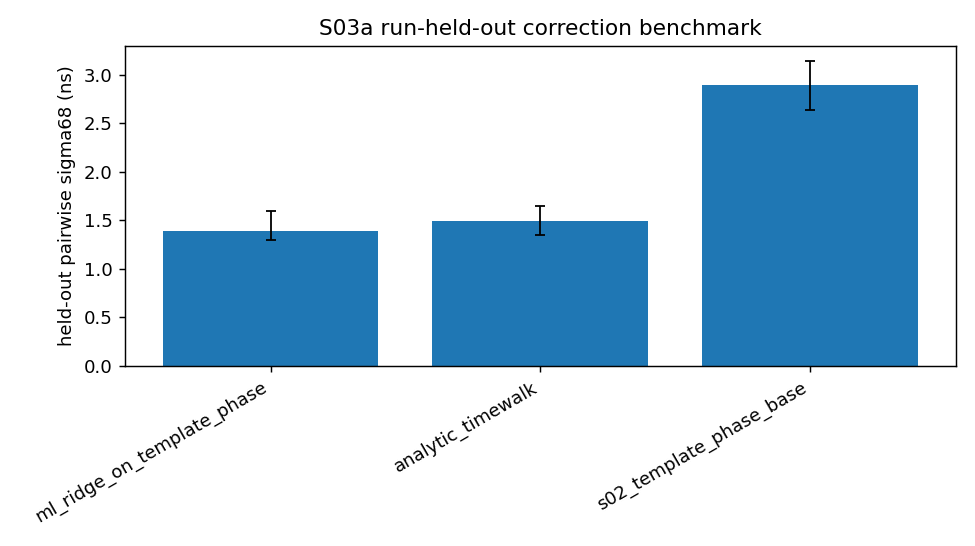
\includegraphics[width=0.78\linewidth]{../figures/reports/1781000705.514827.50025402__s03a_analytic_timewalk_correction/fig_s03a_head_to_head.png}
  \caption{Timing head-to-head from the analytic timewalk closure.  The initial ML gain over a global template is largely closed by an explicit amplitude model.}
\end{figure}

\subsection{The pile-up headline is limited by live-time, not by classifier score}

The most important rate-level revision is that the original \(R_{\max}\) estimate
used \(\tau_{\rm eff}=90\) ns as an assumption.  Direct waveform live-time estimates
do not recover that value.  At the 10\% tail crossing, the traditional template
estimate gives \(124.79\) ns with CI \([123.32,126.33]\) ns, implying a rescaled
combined \(R_{\max}\) near \(3.05\) MHz rather than \(4.22\) MHz.  Scanning the tail
threshold changes the numerical live-time but does not restore a 90 ns measured
window.

For two-pulse recovery, compact MLP/CNN methods can resolve shorter synthetic
separations and reduce timing RMS, but they also raise failure rates.  A representative
template-like injection benchmark found a bounded two-pulse fit live-time of 60 ns
with time RMS \(13.83\) ns and failure rate 0.172, while the compact ML method reached
20 ns with time RMS \(9.41\) ns but failure rate 0.323.  That is a method-ranking
result for controlled injections, not a final real-pile-up measurement.

\begin{figure}[H]
  \centering
  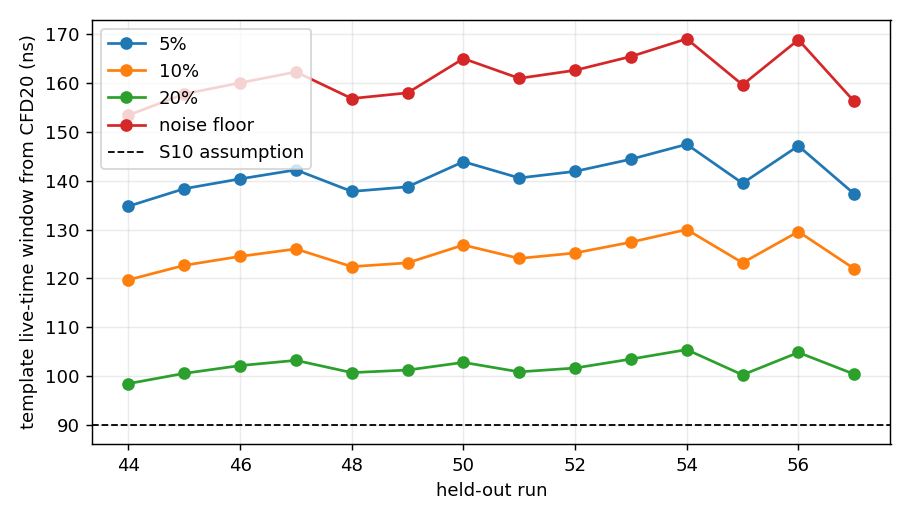
\includegraphics[width=0.82\linewidth]{../figures/reports/1781007337.1308.7dc86005/fig_threshold_scan_by_run.png}
  \caption{Threshold-scan live-time summary.  All tested waveform definitions remain above the 90 ns assumption used by the original rate estimate.}
\end{figure}

\subsection{Pulse shape is compact, and ML wins only in the compact regime}

The pulse-shape representation studies found that the first three PCA components
capture about 89\% of shape variance and eight components capture about 99.7\%.
A small autoencoder beats PCA by 40--51\% in reconstruction MSE for two to four
latent dimensions, but PCA wins at eight dimensions.  The conclusion is not that
the pulse is intrinsically high-dimensional; it is that a compact nonlinear embedding
is a useful summary when downstream tasks need only a few coordinates.

The same line of work is also the programme's clearest leakage lesson.  Learned
representations repeatedly failed to produce robust downstream superiority once
run-family and event-block shuffle controls were applied.  Conversely, shape-only ML
does win on injected corruption labels where the truth is independent of the input
definition.  The distinction is central: ML wins are accepted only when the target is
not a disguised restatement of the feature construction.

\subsection{Shape-dependent amplitude closures are the strongest ML wins}

The largest accepted ML gains are in waveform-shape closures with independent targets.
On duplicate odd-readout amplitude and charge, hist-gradient-boosted trees reduced
held-out amplitude res68 from 0.1238 for calibrated peak amplitude to 0.0091, and
charge res68 from 0.1954 for calibrated integral charge to 0.0151.  On artificial
constant-ceiling saturation, gradient boosting recovered true amplitude at roughly
3--5\% res68, compared with 10--29\% for a fixed-template rising-edge extrapolation.
These are real wins, but their domain is explicit: duplicate-readout and simulated
saturation closure, not absolute per-event beam energy without a truth bridge.

\begin{figure}[H]
  \centering
  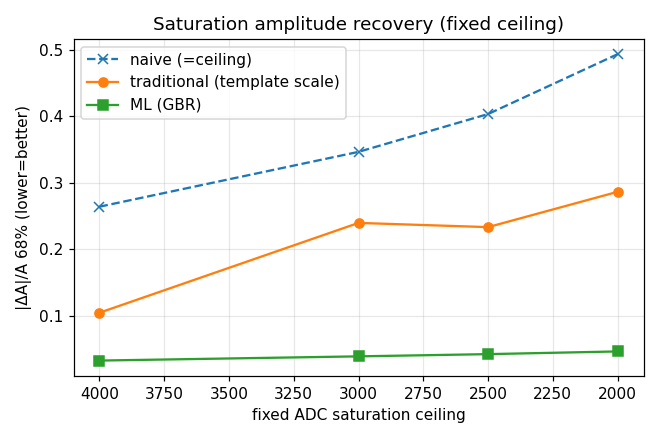
\includegraphics[width=0.78\linewidth]{../figures/reports/P07_saturation_recovery/fig_saturation_recovery.png}
  \caption{Saturation recovery on constant-ceiling artificial clips.  The leakage-fixed gradient-boosted regressor degrades more slowly than the fixed-template extrapolation as clipping becomes more severe.}
\end{figure}

\subsection{Pedestal studies identify a pathology, not a final correction}

The adaptive positivity-constrained pedestal is not validated by its zero-violation
construction.  Against leave-one-pretrigger-out targets on held-out runs 57 and 65,
it has MAE \(341.04\) ADC and mean bias \(-310.69\) ADC; the simple mean/median
baselines are better, and a calibrated HGB regressor reaches MAE \(48.88\) ADC.  The
ML result is useful as a contamination diagnostic, but the current mirror contains no
true forced/random pedestal sample.  The honest conclusion is therefore that large
adaptive lowering tags waveform contamination or pathology until a zero-signal
validation source is found.

\begin{figure}[H]
  \centering
  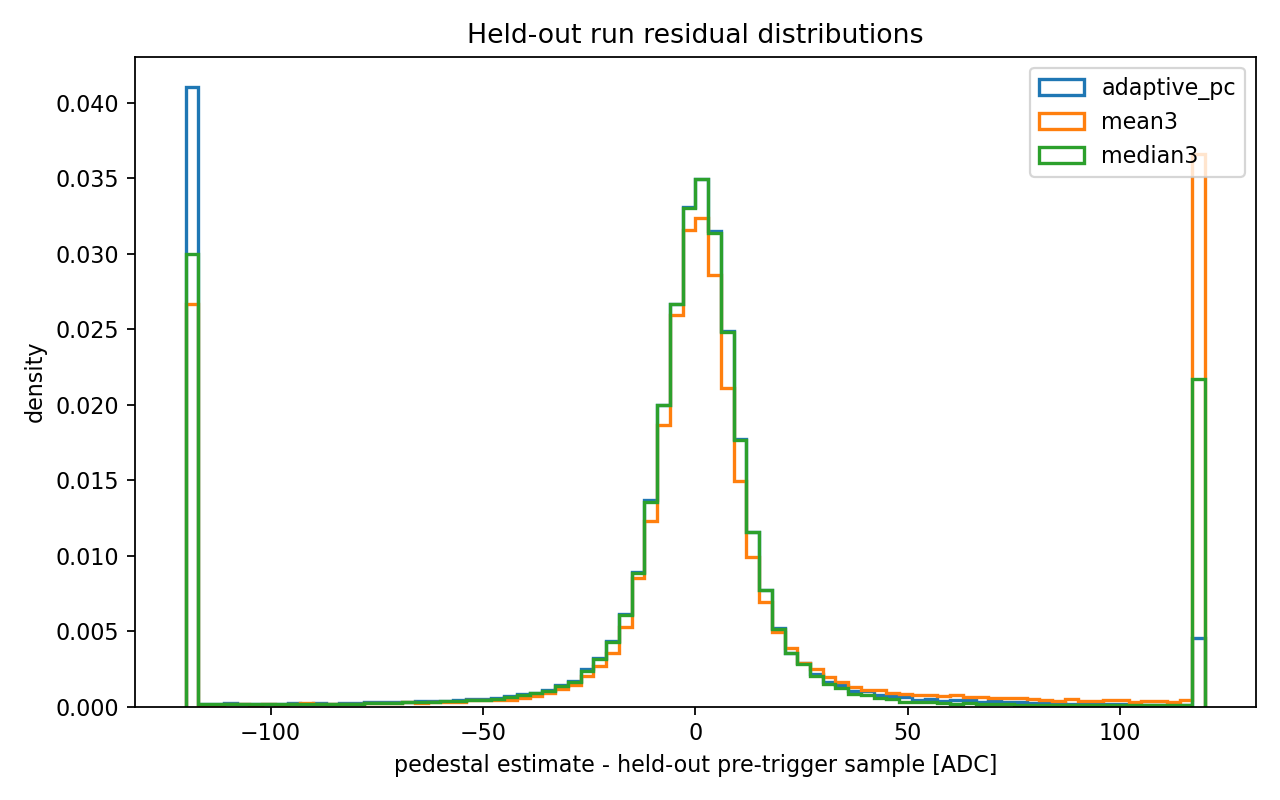
\includegraphics[width=0.78\linewidth]{../figures/reports/1780997954.15337.77205a71__s16_pedestal_baseline_validation/fig_heldout_residual_distributions.png}
  \caption{Held-out pedestal residual distributions.  The adaptive positivity constraint is biased on an independent pretrigger-sample benchmark.}
\end{figure}

\section{Representative numerical verdicts}

\begin{table}[H]
  \centering
  \footnotesize
  \setlength{\tabcolsep}{3pt}
  \begin{tabular}{@{}>{\raggedright\arraybackslash}p{0.12\linewidth}>{\raggedright\arraybackslash}p{0.16\linewidth}>{\raggedright\arraybackslash}p{0.11\linewidth}>{\raggedright\arraybackslash}p{0.34\linewidth}>{\raggedright\arraybackslash}p{0.11\linewidth}@{}}
    \toprule
    Topic & Strong traditional method & ML/NN method & Primary result & Verdict \\
    \midrule
    Timing pickoff & template phase & Ridge on CFD20 & \(2.889\,[2.639,3.205]\) ns vs \(1.846\,[1.521,2.014]\) ns & ML wins initial scan \\
    Analytic timewalk & amplitude timewalk & Ridge residual & \(1.495\,[1.347,1.644]\) ns vs \(1.392\,[1.297,1.596]\) ns & analytic closes most gain \\
    Live-time & template tail & Ridge live-time & \(124.79\,[123.32,126.33]\) ns vs \(123.22\,[120.71,125.61]\) ns & no 90 ns recovery \\
    Two-pulse closure & bounded template fit & compact MLP & 60 ns \([40,60]\), fail 0.172 vs 20 ns \([15,60]\), fail 0.323 & ML RMS win, adoption gated \\
    Duplicate amplitude & calibrated peak & HGB & res68 \(0.1238\,[0.1221,0.1251]\) vs \(0.0091\,[0.0090,0.0093]\) & ML wins \\
    Duplicate charge & calibrated integral & HGB & res68 \(0.1954\,[0.1936,0.1975]\) vs \(0.0151\,[0.0148,0.0153]\) & ML wins \\
    Saturation & rising-edge template & GBR & res68 0.104--0.286 vs 0.032--0.046 & ML wins on clips \\
    Pedestal proxy & mean3 / median3 & calibrated HGBR & MAE \(260.70\,[236.25,287.99]\) vs \(48.88\,[43.82,55.29]\) ADC & ML diagnostic win \\
    \bottomrule
  \end{tabular}
  \caption{Representative head-to-head results.  Bracketed intervals are bootstrap 95\% CIs when reported by the source study.}
\end{table}

\section{GEANT4 and the truth boundary}

The data-only programme has a hard boundary: absolute energy and particle identity
cannot be proven from HRD waveform data alone.  GEANT4 is therefore not an optional
polish step; it is the required truth bridge for deciding whether charge/depth
patterns correspond to proton/deuteron identity and deposited energy.  The first
schema audit showed that the external \texttt{hibeam\_g4} code can be built and can
write a truth tree in a patched smoke run, but the exact supplied production macro was
blocked by an unregistered \texttt{/ElGen/CSFile} command.  That result is valuable
because it turns ``GEANT4 needed'' into a concrete software-interface problem rather
than a vague future task.

A later truth-anchored energy calibration used a high-statistics GEANT4 truth tree as
a layer-level prior rather than an event-aligned truth match.  That model panel is
important because it tested the exact class of methods that might be proposed for a
final energy regressor: ridge, gradient-boosted trees, a tabular MLP, a 1D-CNN, and a
new physics-residual MLP architecture.  The winner was not a neural network.  The
GEANT4 Birks lookup, a traditional truth-anchored calibration, achieved the best
held-out res68.

\begin{table}[H]
  \centering
  \scriptsize
  \begin{tabular}{llll}
    \toprule
    Method & Family & Held-out res68 & Bootstrap 95\% CI \\
    \midrule
    GEANT4 Birks lookup & traditional truth-anchored & 0.04024 & [0.03886, 0.04161] \\
    Gradient-boosted trees & ML tree & 0.05669 & [0.04880, 0.06720] \\
    Physics-residual MLP & new neural residual & 0.05868 & [0.04902, 0.07788] \\
    Ridge & ML linear & 0.09667 & [0.08872, 0.11721] \\
    1D-CNN & neural waveform & 0.26570 & [0.24927, 0.28908] \\
    Old power law & traditional empirical & 0.46236 & [0.44431, 0.56438] \\
    Tabular MLP & neural tabular & 0.69235 & [0.68424, 0.69965] \\
    \bottomrule
  \end{tabular}
  \caption{Truth-anchored energy model panel.  The winner is the traditional GEANT4 Birks lookup; learned methods do not supersede the physics prior in this benchmark.}
\end{table}

\section{Systematics and caveats}

Several systematic limits recur across the programme.  First, run splitting is
necessary but not sufficient.  Some labels, especially \(D_t\), curvature, and
downstream tail definitions, are partly functions of the same waveform features used
by the model.  A classifier can score near perfectly in that setting without
measuring a new physical process.  The accepted criterion is therefore stricter than
held-out performance: a result must also survive shuffle controls, forbidden-feature
audits, and where possible independent or injected truth.

Second, the robust metric and the operational metric can diverge.  In two-pulse
studies, ML improves RMS and resolvability delay but often increases the failure
rate.  A lower RMS conditional on successful reconstruction is not a production win
unless the missing or failed cases remain controlled on real high-current data.

Third, several conclusions are proxy-validations.  Duplicate odd-readout closure is
an independent electronics target, but it is not absolute deposited energy.  Artificial
saturation closure has known truth, but it is not the same as natural digitizer
saturation.  Leave-one-pretrigger-out pedestal validation is independent inside a
beam-triggered pulse, but it is not a forced/random zero-signal sample.  GEANT4 truth
currently supplies a layer-level prior, not event alignment to the HRD data.

Finally, the pile-up rate depends on live-time definition and censoring.  The measured
waveform windows are consistently longer than the 90 ns assumption, but the exact
operational \(R_{\max}\) still depends on threshold choice, acquisition-window
censoring, and how real high-current candidate morphologies map onto true overlapping
pulses.

\section{Open questions}

The first unresolved question is absolute energy and particle identity.  The direct
path is a production GEANT4 sample with validated cross-section handling, material
definitions, Birks response, optical/electronics response where needed, and a documented
mapping from simulated scintillator layers to the HRD B-stack channels.  Until then,
charge/depth labels are useful weak labels, not truth.

The second unresolved question is real pile-up truth.  The programme has strong
synthetic-injection evidence and current-dependent excesses, but no event-level label
stating which beam pulses truly contain two particles.  The next decisive study must
connect high-current waveform taxa, topology, live-time, and either simulation truth
or an independent experimental handle.

The third unresolved question is the pedestal source.  A true forced/random trigger
sample would decide whether the adaptive lowering is an electronics correction or a
contamination flag.  Without it, the safest interpretation is diagnostic.

The fourth unresolved question is transfer.  Many ML wins are real inside their
closure domain; the remaining work is to show that the same methods keep their
advantage under run-family, topology, saturation, and current shifts while preserving
failure-rate and uncertainty calibration.

\section{Final verdict}

The programme does not support a blanket statement that ML is better than traditional
analysis, nor the reverse.  It supports a conditional rule.  ML wins when the truth is
independent and the information is genuinely in waveform shape: duplicate-readout
amplitude/charge, saturation recovery on leakage-free clips, compact low-dimensional
representations, and some injected two-pulse reconstructions.  Traditional or
physics-anchored methods win when the dominant effect has a compact analytic form:
amplitude timewalk, Poisson/live-time rate scaling, and GEANT4 truth-anchored energy
calibration.  The open scientific path is therefore not to replace the analytic
analysis with a black-box model, but to use ML as a shape-sensitive residual tool
inside a reproduce-first, truth-aware calibration chain.

\appendix
\chapter{Method Logic Trace}

This appendix records the reasoning chain behind the analysis choices.  It is
included to make the report auditable: a reader should be able to see not only
what number was quoted, but why that operation was used, what alternative it
guards against, and what interpretation is allowed.

\section{Global rules}

\begin{enumerate}
  \item Start from raw waveforms whenever a population count or selection claim
  matters.  Sorted or derived branches are useful diagnostics, but they can
  encode historical choices that are invisible to a later reader.
  \item Separate deterministic definitions from learned approximations.  If the
  label is exactly \(A>1000\) ADC, a model trained to predict that label is not
  discovering physics; it is approximating the cut.
  \item Compare methods on run-held-out data.  Run period, beam current,
  topology, and calibration are correlated, so random row splits can overstate
  transfer performance.
  \item Accept ML only against a strong traditional comparator on the same
  target, population, split, and metric.  A neural model beating a weak baseline
  does not justify replacing a transparent physics model.
  \item Distinguish construction truth, electronics closure, simulation truth,
  and real-event physics truth.  Injected overlaps, duplicate readout, and
  GEANT4 each answer different questions.
\end{enumerate}

\section{Step-by-step chain}

\begin{longtable}{@{}p{0.06\linewidth}p{0.20\linewidth}p{0.24\linewidth}p{0.24\linewidth}p{0.18\linewidth}@{}}
\toprule
Step & Input & Operation & Reason & Interpretation \\
\midrule
\endhead
1 & Raw B-stack \texttt{HRDv} & Read the 18-sample waveforms for physical even B channels & This is the least ambiguous source for a pulse-count claim & Counts are raw-data anchored \\
2 & Samples 0--3 & Compute \(b=\mathrm{median}(w_0,w_1,w_2,w_3)\) & The median is robust to one bad pre-pulse sample & This is a selection baseline, not final pedestal truth \\
3 & Baseline-subtracted waveform & Compute \(A=\max_j(w_j-b)\) & Peak amplitude is the historical selection scalar & The selected population is deterministic \\
4 & \(A\), stave id & Keep B2/B4/B6/B8 pulses with \(A>1000\) ADC & This defines the reproducible B-stack population & All downstream claims inherit this gate \\
5 & Selected pulses & Build stave- and amplitude-binned templates & Pulse shape changes with stave and amplitude & Template quality is a covariate \\
6 & Leading edge & Compute CFD20 seed time & A fractional crossing gives an interpretable local seed & The seed is a software primitive \\
7 & Template and derivative & Fit sub-sample template phase & Timing needs a local shape model and sample masking & Raw time is model-estimated \\
8 & Amplitude and run structure & Apply timewalk and offsets & Leading-edge time depends on amplitude and calibration period & Analytic timewalk explains most timing gain \\
9 & Corrected stave times & Form inter-stave residuals & Same-particle residuals avoid needing external absolute time truth & B4/B6/B8 define the clean timing reference \\
10 & Residual distribution & Quote \(\sigma_{68}\), core fits, and tails when available & A single Gaussian core hides topology tails & The metric must be named with every claim \\
11 & B2 residuals & Compare topology covariance & B2 has terminal and overlap-dominated populations & B2 broadening is topology-local \\
12 & Occupancy target & Compute \(R_{\max}=\mu_{\max}/\tau_{\mathrm{eff}}\) & Rate limits depend directly on live-time & The 4.22 MHz value assumes 90 ns \\
13 & Waveform tails & Measure live-time from data & The assumed 90 ns window must be tested & The 10-percent estimate implies about 3.05 MHz \\
14 & Current pairs & Compare high-current excess after baseline structure & Real beam pile-up should increase with current & Quote excess, not raw score \\
15 & Injected overlaps & Compare bounded template and ML recovery & Synthetic truth allows controlled method ranking & ML RMS wins require failure-rate gates \\
16 & Waveform matrices & Compare PCA and autoencoder latents & Tests whether pulse shape is low-dimensional & Nonlinearity helps mainly in compact latents \\
17 & Duplicate readout & Predict amplitude and charge closure & The target is independent electronics information & This is not absolute energy truth \\
18 & Artificial clips & Recover unclipped amplitude & Construction truth is known & ML wins artificial saturation closure \\
19 & Pretrigger samples & Validate pedestal estimators & A positivity constraint can pass by construction & Adaptive lowering is a pathology diagnostic \\
20 & GEANT4 truth & Benchmark energy models & Real HRD data lack event-level energy and PID truth & GEANT4 anchors energy interpretation \\
\bottomrule
\end{longtable}

\section{How the conclusions follow}

The selection conclusion follows because the gate contains no trained parameter:
for fixed input bytes and fixed implementation, the row count is a reproducible
integer.  The uncertainty is therefore provenance and implementation risk, not
binomial counting error.

The timing conclusion follows because a stronger analytic amplitude-timewalk
model closes most of the initial ML advantage.  ML residual correction remains a
useful diagnostic, but it is not adopted as the default timing model unless it
wins against the analytic comparator on the same run-held-out benchmark with a
larger and calibrated margin.

The pile-up-rate conclusion follows from the occupancy equation.  The previous
headline was conditional on \(\tau_{\mathrm{eff}}=90\) ns.  Once the waveform
tail measurement gives a longer live-time, the same occupancy requirement
implies a lower admissible rate.  ML classifiers diagnose waveform structure,
but they do not replace the live-time term in the rate equation.

The ML conclusion is task-specific.  ML wins where the target is independent and
shape contains recoverable information, such as duplicate-readout closure and
artificial saturation.  It is rejected or kept diagnostic where the label is a
restatement of the inputs, where leakage risk is high, or where a transparent
physics model already captures the dominant structure.

The energy and PID conclusion follows from missing truth.  HRD waveform data can
support sample-level enrichment and closure tests, but they do not contain
event-level particle identity or deposited-energy truth.  GEANT4 is therefore
the required bridge for physics-facing energy and PID claims.

\section{Future edit checklist}

Any future change to a headline number must update the source study reference,
the Markdown summary, the LaTeX chapter, the visual figure or table, the
validation command, and the caveat that bounds the interpretation.  This prevents
a table from changing while the reasoning chain remains stale.

\end{document}
